\documentclass[12pt,xcolor=dvipsnames,professionalfonts]{beamer}

% Pakete
\usepackage[utf8]{inputenc}
\usepackage[ngerman]{babel}

% AMS Pakete
\usepackage{amsmath}
\usepackage{amsfonts}
\usepackage{amssymb}

\usepackage{booktabs}
\usepackage{multirow}
\usepackage{array}
\usepackage[percent]{overpic}

% Einheiten
\usepackage{siunitx}
\sisetup{
	output-decimal-marker={,},
	separate-uncertainty
}

% Grafiken
\usepackage{graphicx}
\usepackage{tabularx}
\setbeamerfont{caption}{size=\footnotesize}
\setbeamertemplate{caption}{\raggedright\insertcaption\par}

\newcommand{\todo}[1]{{\textcolor{Green}{(#1)}}}

% Theme
\usetheme{Boadilla}
\usecolortheme{rose}
\useoutertheme{infolines}
\useinnertheme{rectangles}
\setbeamertemplate{itemize subitem}[triangle]

\usefonttheme[onlymath]{serif}

% [num] Zitationen
\setbeamertemplate{bibliography item}[text]

% Navigationsleiste ausschalten
\beamertemplatenavigationsymbolsempty

\author[Christopher Deutsch]
{Christopher Deutsch}

\title
{Störkörpermessung an Hohlraumresonatoren}

\subtitle
{}
%\logo{}

\institute[]
{Physikalisches Institut der Universität Bonn\\
Seminar zur Bachelorarbeit}

\date{24. September 2015}

%\setbeamercovered{transparent}
%\setbeamertemplate{navigation symbols}{}

\newcommand{\beginbackup}{
	\newcounter{framenumbervorappendix}
	\setcounter{framenumbervorappendix}{\value{framenumber}}
}
\newcommand{\backupend}{
	\addtocounter{framenumbervorappendix}{-\value{framenumber}}
	\addtocounter{framenumber}{\value{framenumbervorappendix}} 
}

\begin{document}
\maketitle

\begin{frame}{Inhalt}
	\tableofcontents
\end{frame}

\section{Motivation}
%\frame{\tableofcontents[currentsection]} Inhaltsverzeichnis für die aktuelle Section
% \setlength\itemsep{1em} in itemization zur abstandeinstellung
\begin{frame}{Motivation}
	\begin{itemize}
		\item Begrenzung des internen Strahlstroms an ELSA
		\begin{itemize}
			\setlength\itemsep{0.25em}
			\item max.\ interner Strahlstrom  $\sim\SI{20}{mA}$ bei \SI{3.2}{GeV}
		\end{itemize}
		\vfill
		
		\item Erweiterung des Stretcherrings durch zweite HF-Station
		\begin{itemize}
			\setlength\itemsep{0.25em}
			\item Klystron und zwei 7-zellige PETRA-Resonatoren
			\item interne Strahlströme bis zu \SI{200}{mA}
		\end{itemize}
		\vfill
		
		\item Bestimmung der elektrischen Feldverteilung durch Störkörpermessung
		\begin{itemize}
			\setlength\itemsep{0.25em}
			\item Beschleunigungsspannung und Shuntimpedanz
			\item Moden höherer Ordnung
		\end{itemize}
	\end{itemize}
\end{frame}


\section{Hohlraumresonatoren}

\begin{frame}{Felder und Schwingungsmoden}
	\begin{columns}[T]
		\column{0.60\textwidth}
		\begin{itemize}
			\item Hohlraum mit leitenden Wänden
			\begin{itemize}
				\setlength\itemsep{0.25em}
				
				\item stehende em.\ Wellen
				
				\item Randbedingungen:
				\begin{align*}
				E_\parallel = 0 \qquad B_\perp = 0
				\end{align*}
				
				\item erlauben nur bestimmte Feldkonfigurationen (Moden)
			\end{itemize}
		\end{itemize}
		\column{0.4\textwidth}
		\centering
		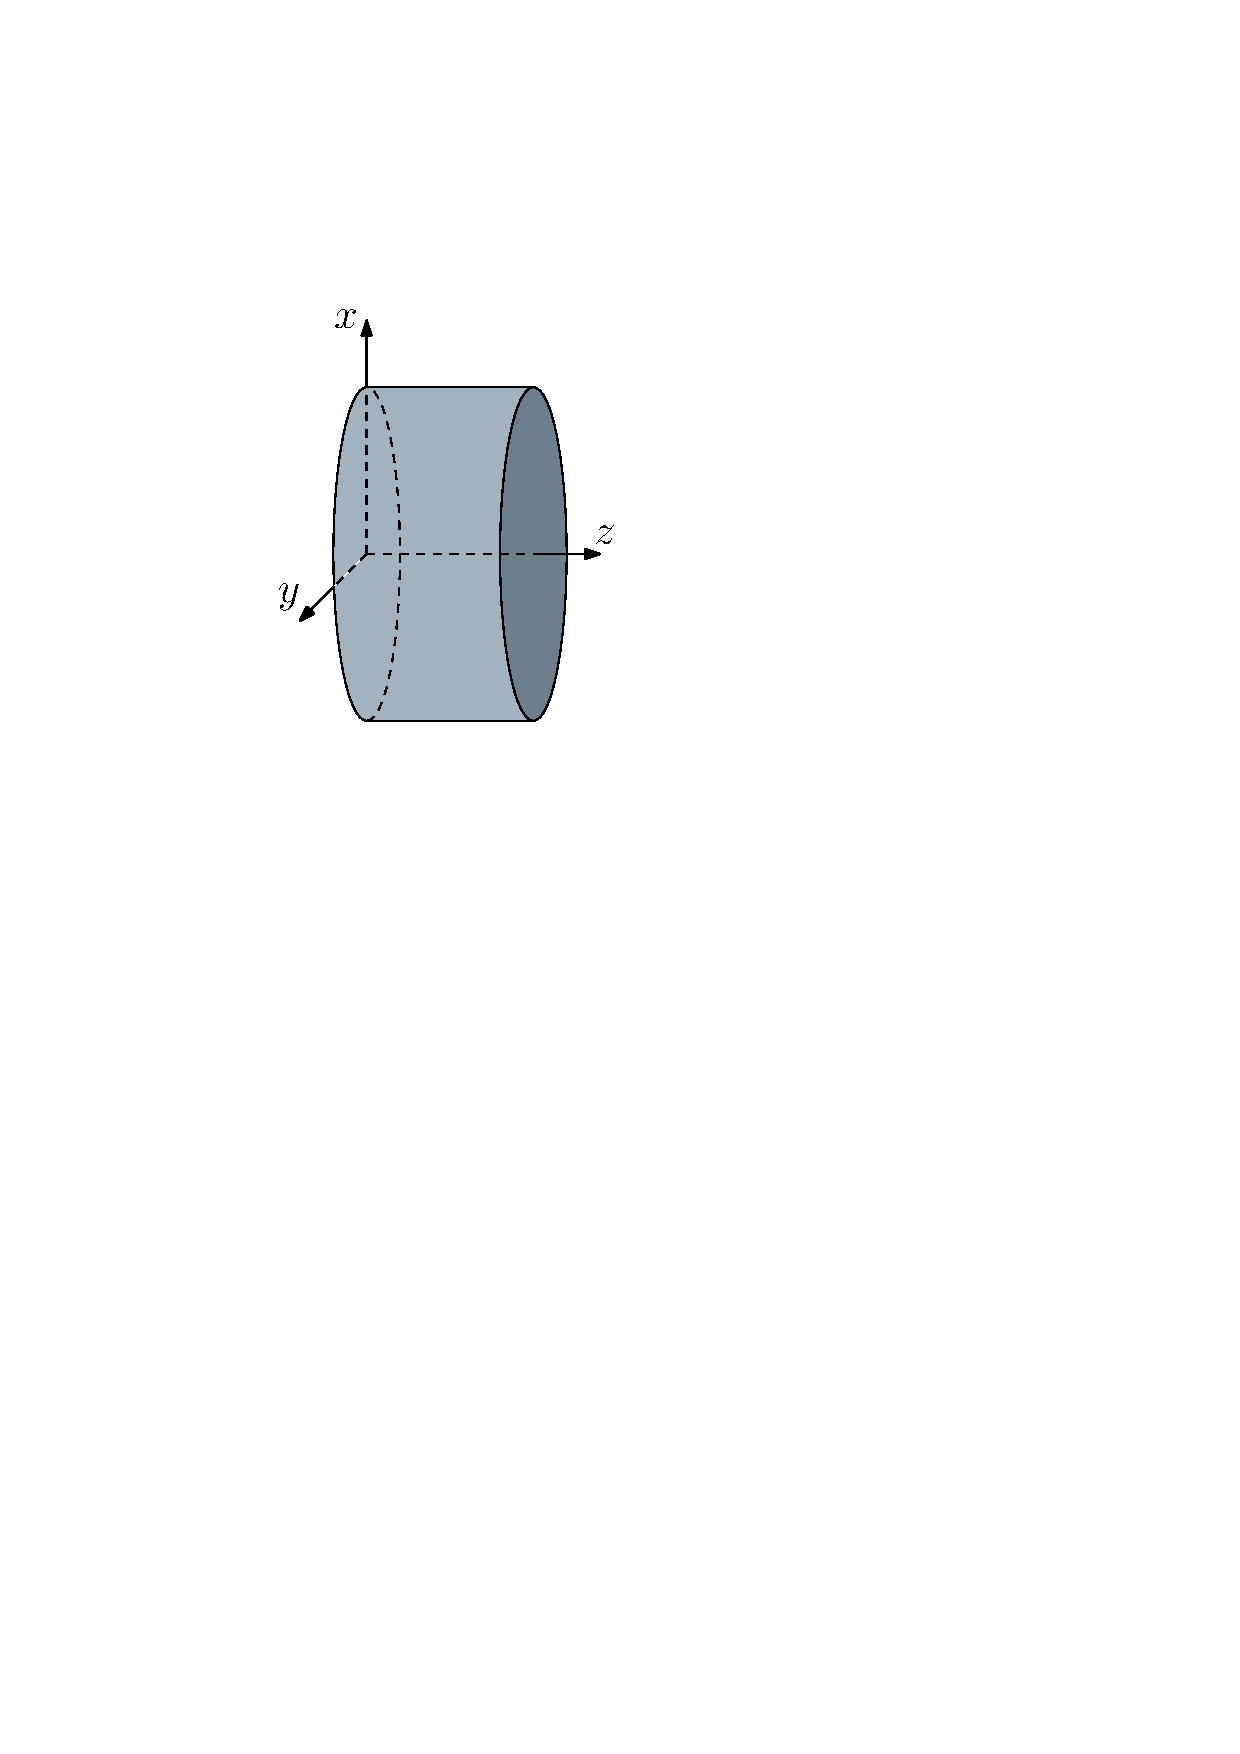
\includegraphics[scale=0.6]{./figures/pillbox.pdf}
	\end{columns}
	\vfill
	\begin{itemize}
		\item zylindersymmetrische Resonatormoden
		\begin{itemize}
			\setlength\itemsep{0.25em}
			\item TM und TE-Moden
			\item Bezeichnung durch drei Indizes $m, n, p$
		\end{itemize}
		
	\end{itemize}
\end{frame}

\begin{frame}{Impedanzmodell für Hohlraumresonatoren}
	\begin{columns}[c]
		\column{0.7\textwidth}
		\begin{itemize}
			\item Parallelschwingkreis als Modell für Hohlraumresonatoren
			\begin{itemize}
				\setlength\itemsep{0.25em}
				\item gültig in der Nähe einer Resonanz
				
				\item beschrieben durch Eigenfrequenz $\omega_0$, Kreisgüte $Q_0$, Shuntimpedanz $R_\mathrm{S}$
			\end{itemize}
		\end{itemize}
		
		\column{0.3\textwidth}
		\centering
		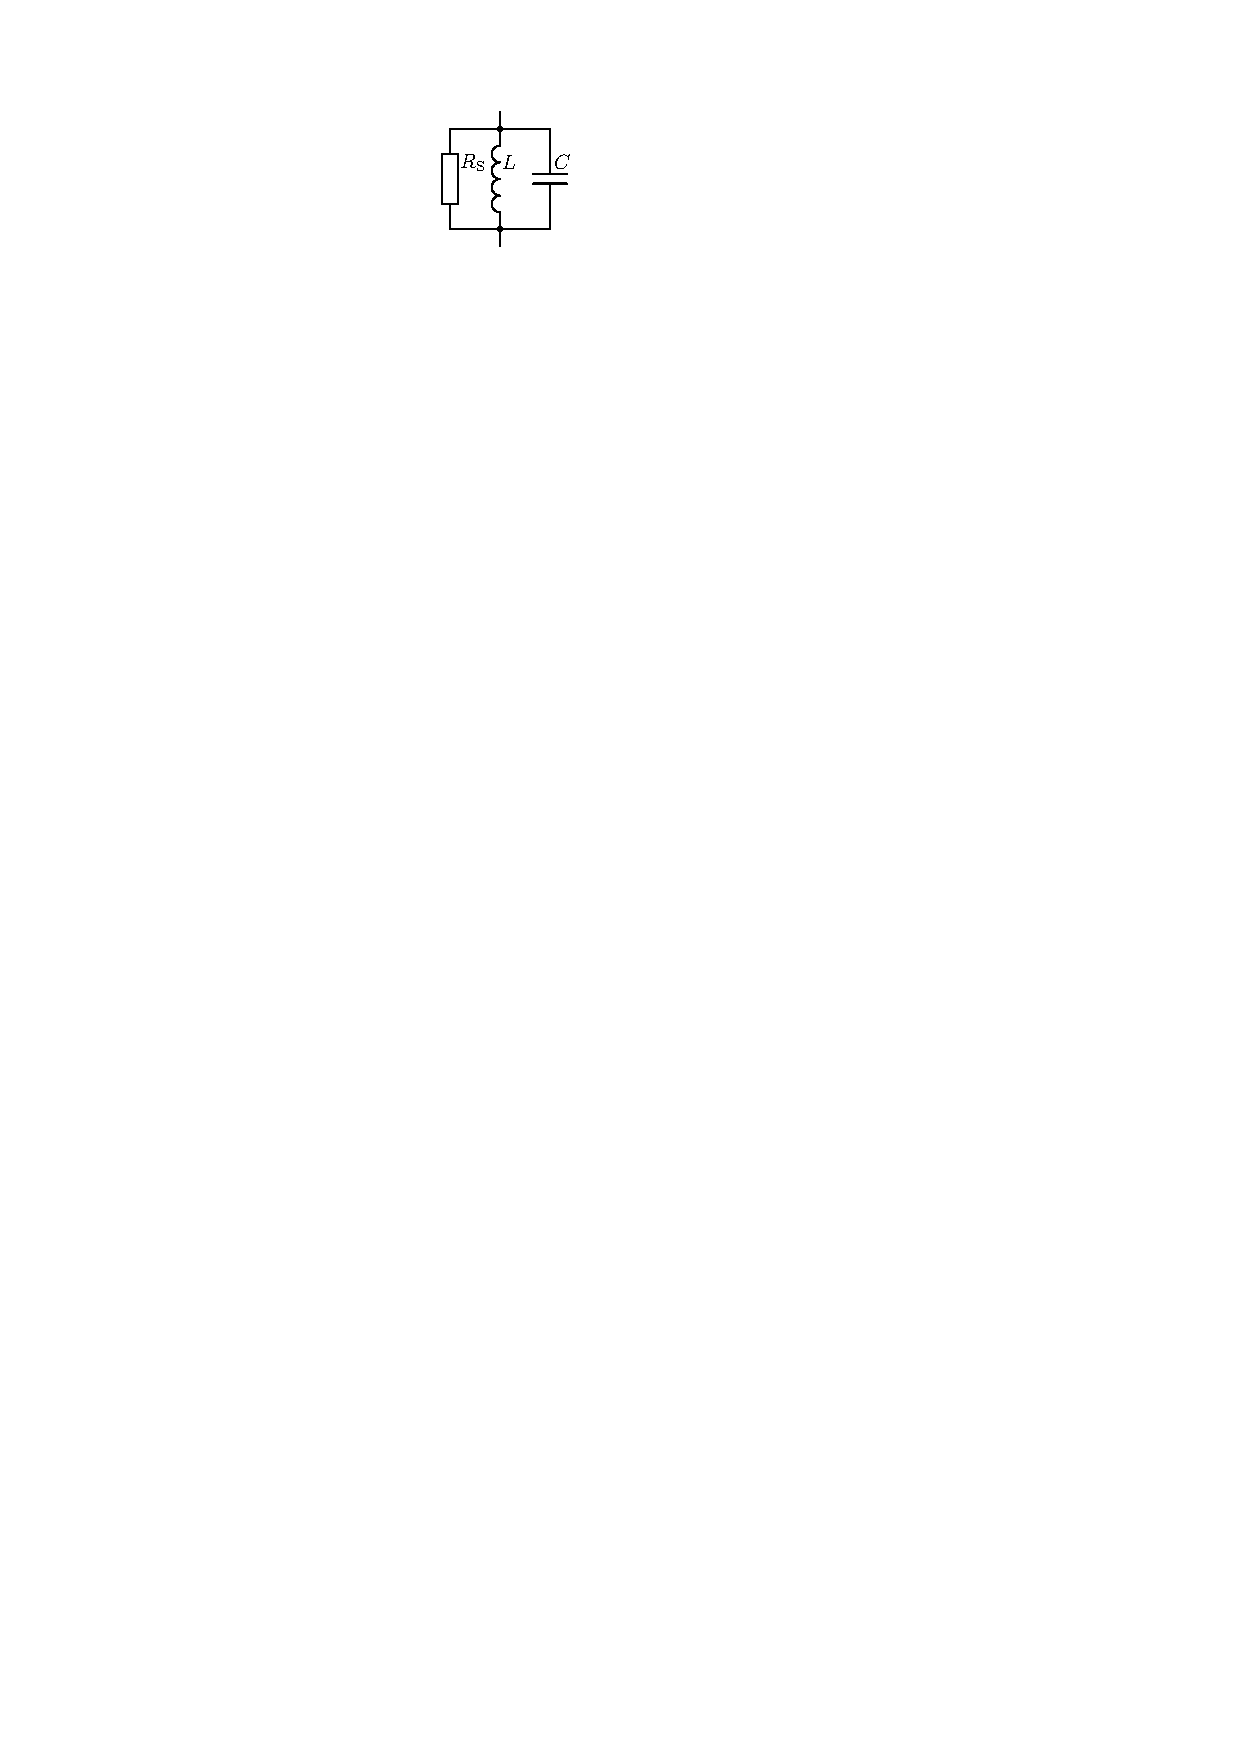
\includegraphics[scale=1.15]{./figures/RLC_circuit.pdf}
	\end{columns}
	\vfill
	\begin{columns}[T]
		\column{0.55\textwidth}
		\begin{itemize}
			\item Impedanzmodell:
			\begin{align*}
			Z(\omega) = \frac{R_\mathrm{S}}{1 + \mathrm{i} Q_0 \left( \frac{\omega}{\omega_0} - \frac{\omega_0}{\omega} \right)}
			\end{align*}
		\end{itemize}
		
		\column{0.45\textwidth}
		\begin{itemize}
			\item mittlere Verlustleistung:
			\begin{align*}
				P_\mathrm{V} = \frac{\left|U\right|^2}{2 R_\mathrm{S}}
			\end{align*}
		\end{itemize}
	\end{columns}
	

\end{frame}

\begin{frame}{Kopplung mit externer Leistungsquelle}
	\begin{columns}[c]
		\column{0.65\textwidth}
		\begin{itemize}
			\setlength\itemsep{1.25em}
			\item Übertragung von Energie in Resonatormode
			\begin{itemize}
				\setlength\itemsep{0.25em}
				\item induktive Schleifenkopplung
			\end{itemize}
			
			\item Kopplung an die äußere Beschaltung
			\begin{itemize}
				\setlength\itemsep{0.25em}
				\item Transformation der Impedanz $Z \rightarrow Z^\prime$
				\begin{align*}
					Z^\prime(\omega) \propto Z(\omega)
				\end{align*}
			\end{itemize}
			
			\item Koppelfaktor $\kappa$:
			\begin{itemize}
				\setlength\itemsep{0.25em}
				\item Maß für Kopplung zwischen Wellenleiter und Resonator\setlength\itemsep{0.25em}
			\end{itemize}
		\end{itemize}
		
		\column{0.35\textwidth}
		\centering
		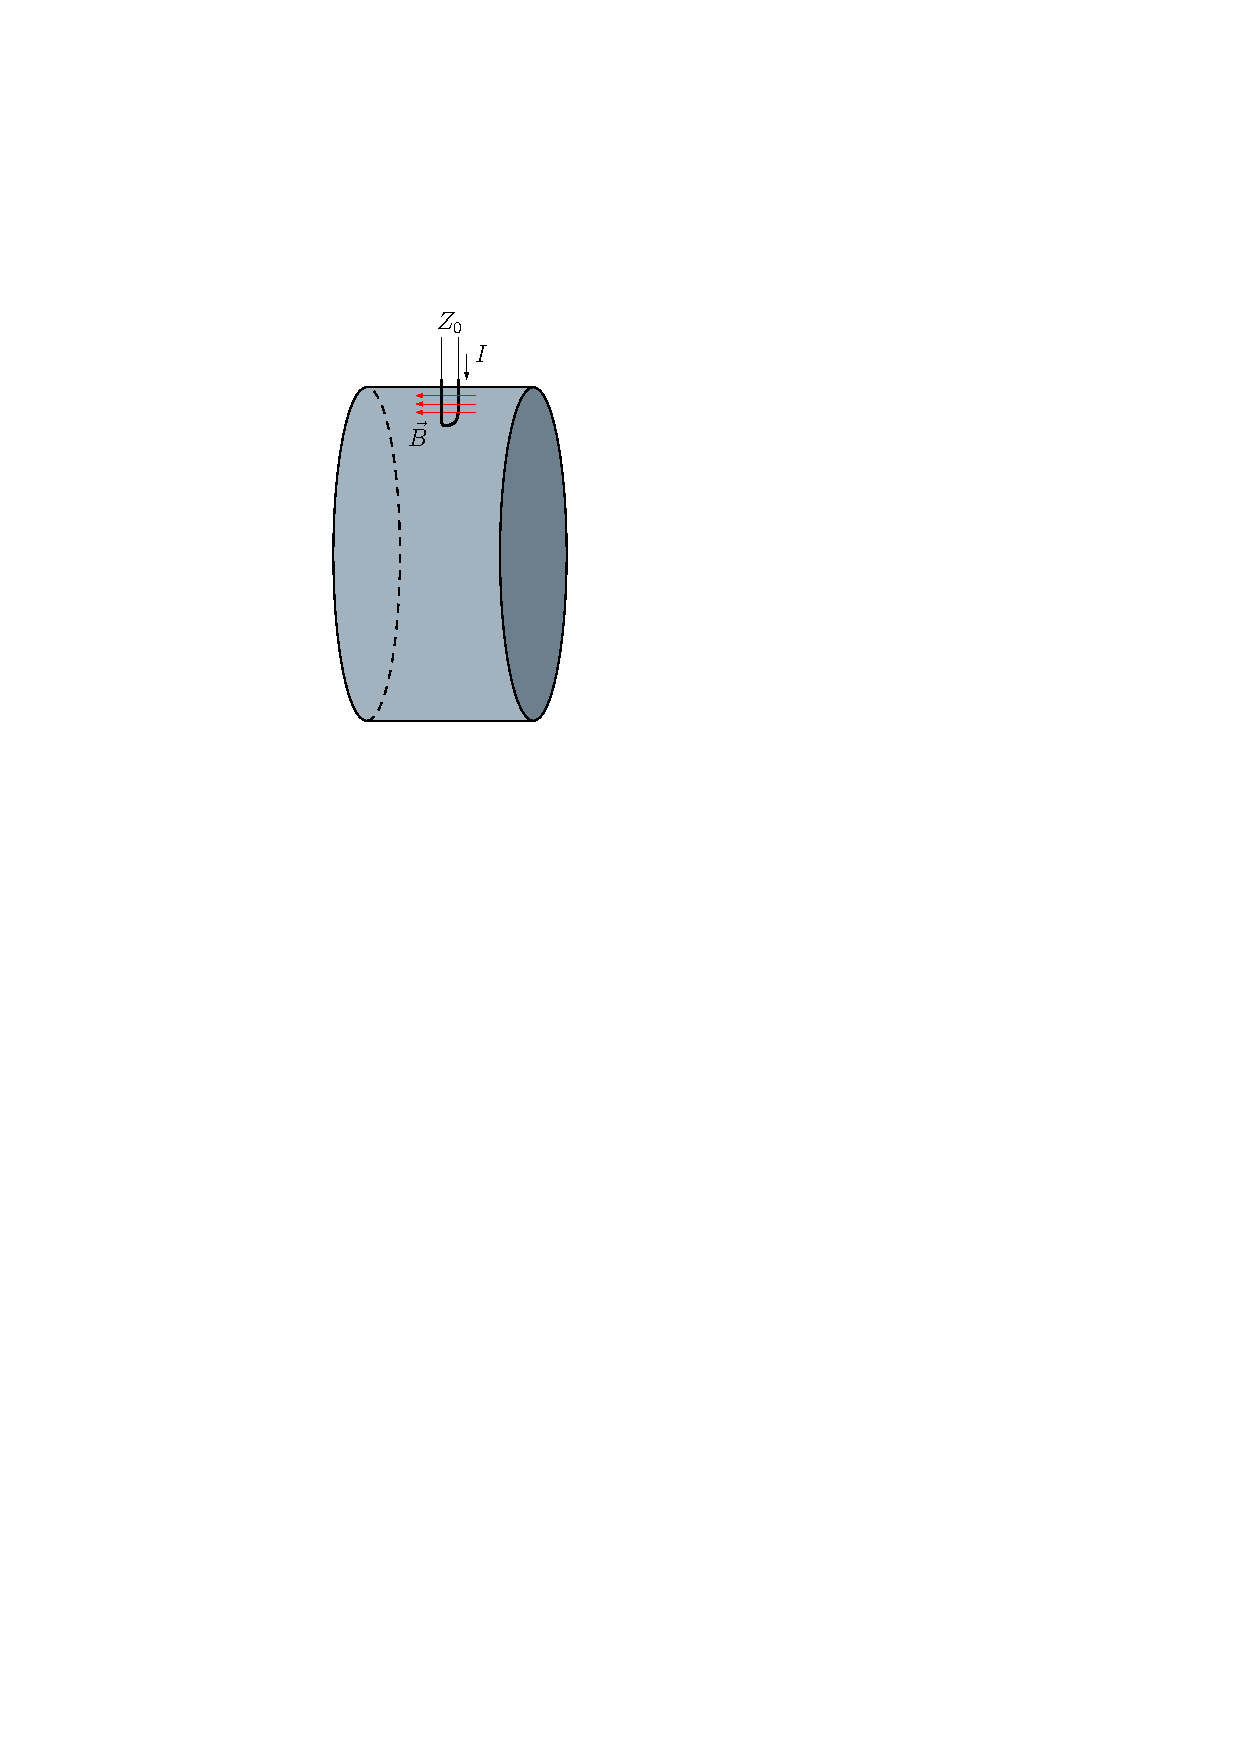
\includegraphics[scale=0.8]{./figures/pillbox_loop.pdf}
	\end{columns}
	
\end{frame}

\begin{frame}
	\begin{itemize}
		\item komplexer Reflexionsfaktor:
		\begin{align*}
		\rho(\omega) = \frac{(\kappa - 1) + \mathrm{i} Q_0 \left(\frac{\omega}{\omega_0} - \frac{\omega_0}{\omega}\right) }{(\kappa + 1) + \mathrm{i} Q_0 \left( \frac{\omega}{\omega_0} - \frac{\omega_0}{\omega} \right)}
		\end{align*}
	\end{itemize}
	\vfill
	\begin{columns}[c]
		\column{0.7\textwidth}
			\begin{small}
				\centering
				% GNUPLOT: LaTeX picture with Postscript
\begingroup
  \makeatletter
  \providecommand\color[2][]{%
    \GenericError{(gnuplot) \space\space\space\@spaces}{%
      Package color not loaded in conjunction with
      terminal option `colourtext'%
    }{See the gnuplot documentation for explanation.%
    }{Either use 'blacktext' in gnuplot or load the package
      color.sty in LaTeX.}%
    \renewcommand\color[2][]{}%
  }%
  \providecommand\includegraphics[2][]{%
    \GenericError{(gnuplot) \space\space\space\@spaces}{%
      Package graphicx or graphics not loaded%
    }{See the gnuplot documentation for explanation.%
    }{The gnuplot epslatex terminal needs graphicx.sty or graphics.sty.}%
    \renewcommand\includegraphics[2][]{}%
  }%
  \providecommand\rotatebox[2]{#2}%
  \@ifundefined{ifGPcolor}{%
    \newif\ifGPcolor
    \GPcolortrue
  }{}%
  \@ifundefined{ifGPblacktext}{%
    \newif\ifGPblacktext
    \GPblacktexttrue
  }{}%
  % define a \g@addto@macro without @ in the name:
  \let\gplgaddtomacro\g@addto@macro
  % define empty templates for all commands taking text:
  \gdef\gplbacktext{}%
  \gdef\gplfronttext{}%
  \makeatother
  \ifGPblacktext
    % no textcolor at all
    \def\colorrgb#1{}%
    \def\colorgray#1{}%
  \else
    % gray or color?
    \ifGPcolor
      \def\colorrgb#1{\color[rgb]{#1}}%
      \def\colorgray#1{\color[gray]{#1}}%
      \expandafter\def\csname LTw\endcsname{\color{white}}%
      \expandafter\def\csname LTb\endcsname{\color{black}}%
      \expandafter\def\csname LTa\endcsname{\color{black}}%
      \expandafter\def\csname LT0\endcsname{\color[rgb]{1,0,0}}%
      \expandafter\def\csname LT1\endcsname{\color[rgb]{0,1,0}}%
      \expandafter\def\csname LT2\endcsname{\color[rgb]{0,0,1}}%
      \expandafter\def\csname LT3\endcsname{\color[rgb]{1,0,1}}%
      \expandafter\def\csname LT4\endcsname{\color[rgb]{0,1,1}}%
      \expandafter\def\csname LT5\endcsname{\color[rgb]{1,1,0}}%
      \expandafter\def\csname LT6\endcsname{\color[rgb]{0,0,0}}%
      \expandafter\def\csname LT7\endcsname{\color[rgb]{1,0.3,0}}%
      \expandafter\def\csname LT8\endcsname{\color[rgb]{0.5,0.5,0.5}}%
    \else
      % gray
      \def\colorrgb#1{\color{black}}%
      \def\colorgray#1{\color[gray]{#1}}%
      \expandafter\def\csname LTw\endcsname{\color{white}}%
      \expandafter\def\csname LTb\endcsname{\color{black}}%
      \expandafter\def\csname LTa\endcsname{\color{black}}%
      \expandafter\def\csname LT0\endcsname{\color{black}}%
      \expandafter\def\csname LT1\endcsname{\color{black}}%
      \expandafter\def\csname LT2\endcsname{\color{black}}%
      \expandafter\def\csname LT3\endcsname{\color{black}}%
      \expandafter\def\csname LT4\endcsname{\color{black}}%
      \expandafter\def\csname LT5\endcsname{\color{black}}%
      \expandafter\def\csname LT6\endcsname{\color{black}}%
      \expandafter\def\csname LT7\endcsname{\color{black}}%
      \expandafter\def\csname LT8\endcsname{\color{black}}%
    \fi
  \fi
    \setlength{\unitlength}{0.0500bp}%
    \ifx\gptboxheight\undefined%
      \newlength{\gptboxheight}%
      \newlength{\gptboxwidth}%
      \newsavebox{\gptboxtext}%
    \fi%
    \setlength{\fboxrule}{0.5pt}%
    \setlength{\fboxsep}{1pt}%
\begin{picture}(4534.00,2834.00)%
    \gplgaddtomacro\gplbacktext{%
      \csname LTb\endcsname%
      \put(814,704){\makebox(0,0)[r]{\strut{}0{,}0}}%
      \put(814,1077){\makebox(0,0)[r]{\strut{}0{,}2}}%
      \put(814,1450){\makebox(0,0)[r]{\strut{}0{,}4}}%
      \put(814,1823){\makebox(0,0)[r]{\strut{}0{,}6}}%
      \put(814,2196){\makebox(0,0)[r]{\strut{}0{,}8}}%
      \put(814,2569){\makebox(0,0)[r]{\strut{}1{,}0}}%
      \put(946,484){\makebox(0,0){\strut{}0{,}99}}%
      \put(2542,484){\makebox(0,0){\strut{}1{,}00}}%
      \put(4137,484){\makebox(0,0){\strut{}1{,}01}}%
    }%
    \gplgaddtomacro\gplfronttext{%
      \csname LTb\endcsname%
      \put(176,1636){\rotatebox{-270}{\makebox(0,0){\strut{}$|\rho|$}}}%
      \put(2541,154){\makebox(0,0){\strut{}$\frac{\omega}{\omega_0}$}}%
    }%
    \gplbacktext
    \put(0,0){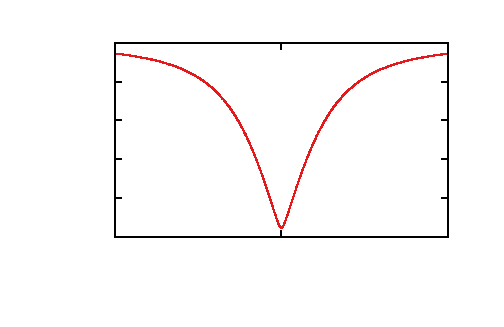
\includegraphics{./plots/resonanzkurve_2}}%
    \gplfronttext
  \end{picture}%
\endgroup

			\end{small}		
		\column{0.3\textwidth}
		\vspace*{-1.3cm}
		\begin{flalign*}
			Q_0 &= 300 &\\
			\kappa &= 1{,}1 &
		\end{flalign*}
	\end{columns}
\end{frame}
	

\section{Resonante Störkörpermessung}

\begin{frame}{Resonante Störkörpermessung}
	\begin{itemize}
		\item Bestimmung von el.\ und mag.\ Feldamplituden in Resonatoren
	\end{itemize}
	\vspace*{0.12cm}
	\begin{columns}[c,onlytextwidth]
		\column{0.6\textwidth}
		\begin{itemize}
			\setlength\itemsep{1.25em}
			\item lokalisierte Störung der Felder durch diel.\ oder mag.\ Störkörper
			\begin{itemize}
				\item Polarisation / Magnetisierung durch äußeres Feld
			\end{itemize}
			
			\item Annahme: kleine Störkörper

			\item Störung abhängig von Feld am Ort des Störkörpers
		
	\end{itemize}
		\column{0.4\textwidth}
		\centering
		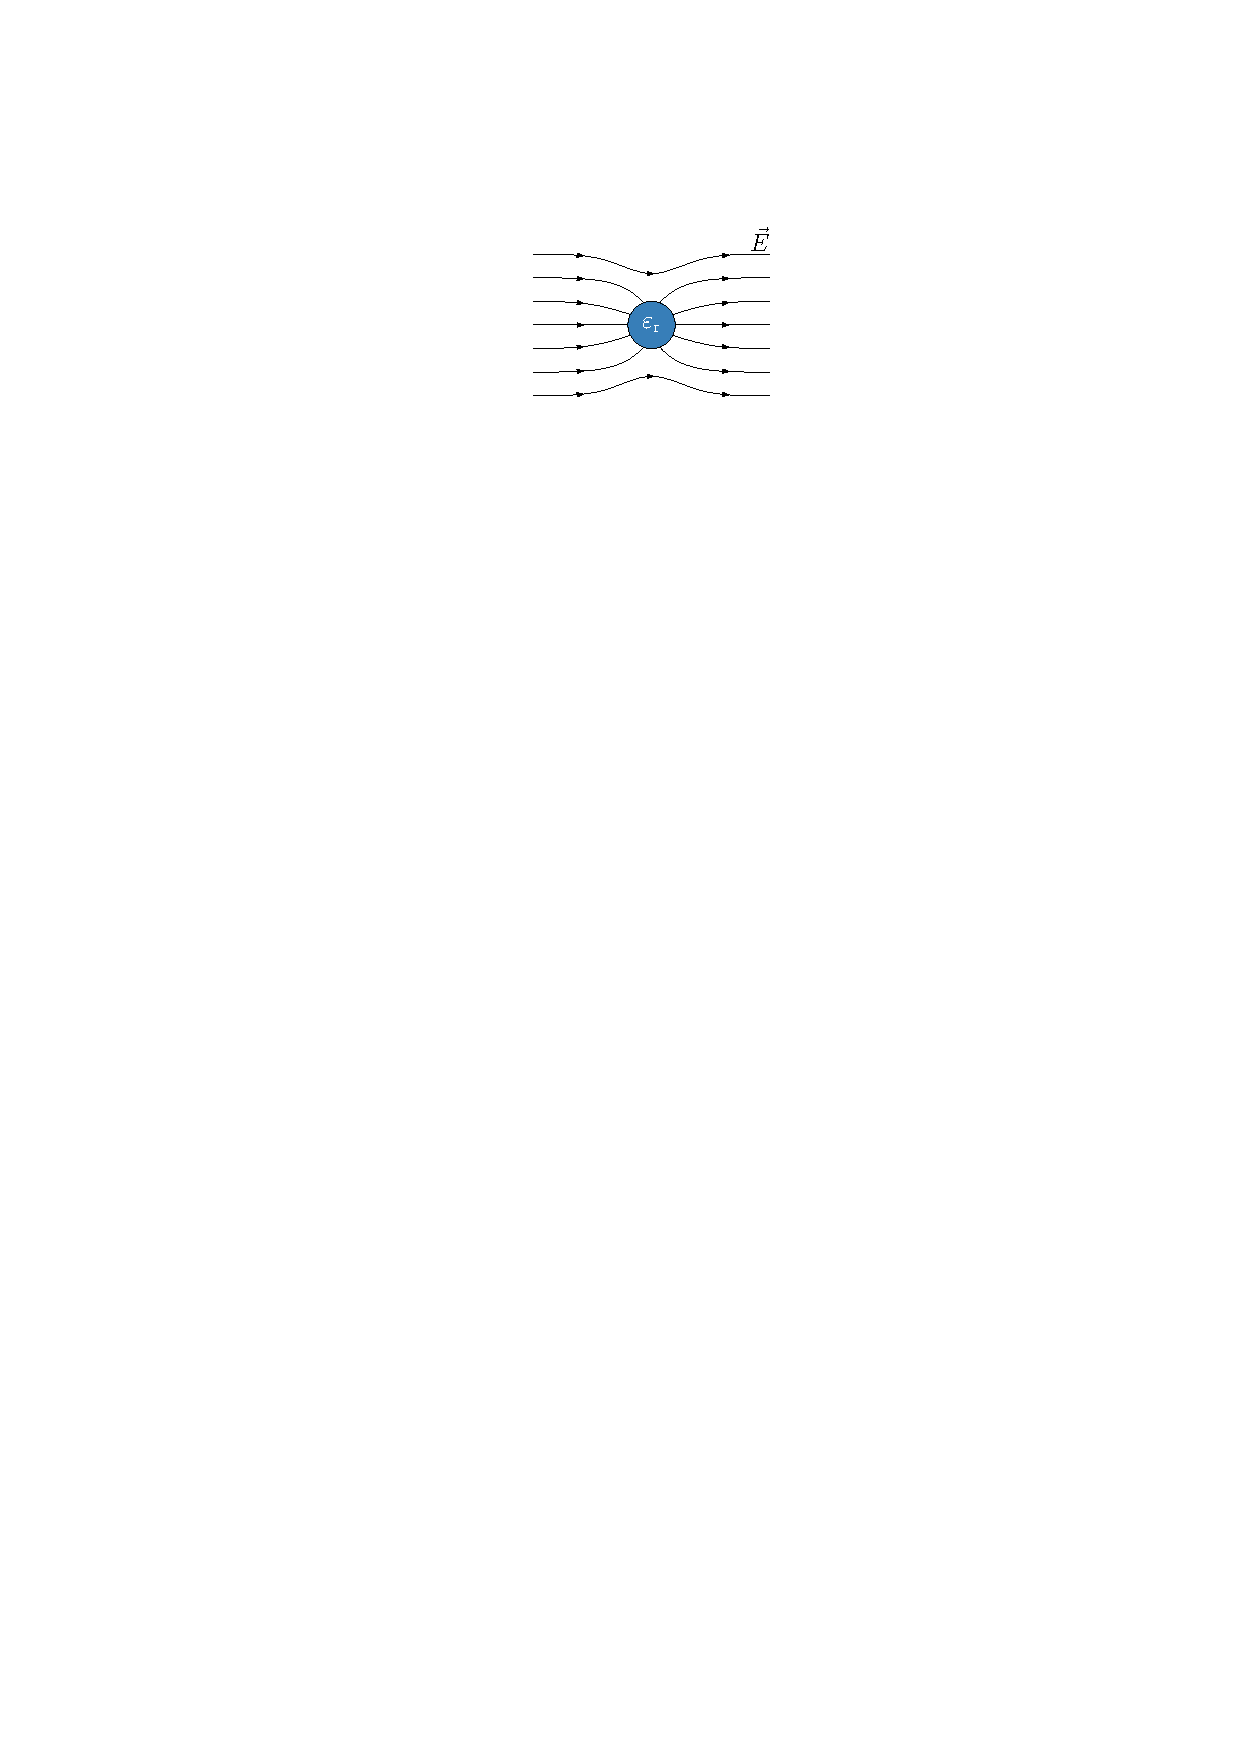
\includegraphics[scale=1.0]{./figures/stoerung.pdf}
		
	\end{columns}

\end{frame}

\begin{frame}
	\begin{itemize}
		\setlength\itemsep{1.25em}
		\item Verschiebung der Resonanzfrequenz:
		\begin{align*}
			\frac{\Delta \omega}{\omega_0} = -\frac{\int_{V} \, \mathrm{d}V \left[ \textcolor{Green}{\vec{E}_0^*} \cdot \textcolor{Red}{\vec{P}} + \textcolor{Green}{\vec{B}_0^*} \cdot \textcolor{Red}{\vec{M}} \right]}{4 W_0}
		\end{align*}
	
	\item Polarisation $\textcolor{Red}{\vec{P}}$ und Magnetisierung $\textcolor{Red}{\vec{M}}$ abhängig von:
		\begin{itemize}
			\setlength\itemsep{0.25em}
			\item Material und Form des Störkörpers
			\item Position des Störkörpers
		\end{itemize}
	\item Bestimmung der ortsabh.\ Feldamplituden des ungestörten Resonators möglich	
	\end{itemize}
\end{frame}

\begin{frame}
	\begin{itemize}
		\setlength\itemsep{1.25em}
		\item el.\ Feldamplitude für dielektrische Störkörper ($\vec{M} = 0$):
		\begin{align*}
			|\vec{E}_0(\textcolor{Red}{\vec{x}_\mathrm{s}})| = \sqrt{- 4 \cdot \frac{W_0}{\textcolor{Red}{\alpha_\mathrm{s}}} \cdot \frac{\textcolor{Red}{\Delta \omega}}{\omega_0}} \quad \text{für} \quad \Delta \omega \leq 0
		\end{align*}
		
		\item Störkörperkonstante $\alpha_\mathrm{s}$ (abh.\ von Form, Permittivität)
	\end{itemize}
\end{frame}

\section{Störkörpermessungen an PETRA-Resonatoren}

\begin{frame}{PETRA-Resonator}
	\begin{figure}
		\centering
		\includegraphics[scale=0.6]{./figures/cavity.pdf}
	\end{figure}
	
	\begin{itemize}
		\setlength\itemsep{1.0em}
		\item Beschleunigung ultrarelativistischer Teilchen durch $\mathrm{TM}_{010}$-Mode bei $\nu_0 = \SI{499.67}{MHz}$
		
		\item Anregung der (gekoppelten) Zellen durch Koppelschleife
		
		\item Abstimmstempel zur Frequenzeinstellung
		
	\end{itemize}
\end{frame}

\begin{frame}{Störkörpermessstand}
	\begin{figure}
		\centering
		\includegraphics[width=1.\textwidth]{./figures/messaufbau.pdf}
	\end{figure}
	\begin{itemize}
		\setlength\itemsep{0.5em}
		\item Schrittmotor zur Bewegung des Störkörpers im Resonator
		\item vektorieller Netzwerkanalysator an Koppelschleife
		\begin{itemize}
			\item Anregung durch Hochfrequenzsignal
			\item Messung des (komplexen) Reflexionsfaktors
		\end{itemize}
		\item automatisierte Messung
	\end{itemize}	
\end{frame}

\begin{frame}{Temperaturabhängigkeit}
	\begin{itemize}
		\setlength\itemsep{1.25em}
		\item Vermessung mit kleiner Schrittweite
		\begin{itemize}
			\setlength\itemsep{0.25em}
			\item Messdauer: $\sim \SI{2}{\hour}$
			\item Temperaturänderung nicht zu vermeiden
		\end{itemize}
		
		\item Resonanzfrequenz sensitiv auf Temperaturänderung \cite{desy_petra7}: 
		\begin{align*}
			\frac{\Delta \nu}{\Delta T} \approx \SI{8}{\kilo\hertz\per\celsius}
		\end{align*}
		
		\item typische Frequenzverschiebung durch Störkörper:
		\begin{align*}
			\Delta \nu \sim \SI{10}{\kilo\hertz}
		\end{align*}
		
		\item \textbf{Lösung:} messe Frequenzen relativ zu einer Referenzfrequenz
		
	\end{itemize}
\end{frame}


\begin{frame}{Messablauf}
	\vspace*{2cm}
	\centering
	\begin{overpic}[width=0.95\textwidth,tics=10]{./figures/messaufbau_refpos.pdf}
		\put (45,20) {
				\fcolorbox{Black}{White}{% GNUPLOT: LaTeX picture with Postscript
\begingroup
  \makeatletter
  \providecommand\color[2][]{%
    \GenericError{(gnuplot) \space\space\space\@spaces}{%
      Package color not loaded in conjunction with
      terminal option `colourtext'%
    }{See the gnuplot documentation for explanation.%
    }{Either use 'blacktext' in gnuplot or load the package
      color.sty in LaTeX.}%
    \renewcommand\color[2][]{}%
  }%
  \providecommand\includegraphics[2][]{%
    \GenericError{(gnuplot) \space\space\space\@spaces}{%
      Package graphicx or graphics not loaded%
    }{See the gnuplot documentation for explanation.%
    }{The gnuplot epslatex terminal needs graphicx.sty or graphics.sty.}%
    \renewcommand\includegraphics[2][]{}%
  }%
  \providecommand\rotatebox[2]{#2}%
  \@ifundefined{ifGPcolor}{%
    \newif\ifGPcolor
    \GPcolortrue
  }{}%
  \@ifundefined{ifGPblacktext}{%
    \newif\ifGPblacktext
    \GPblacktexttrue
  }{}%
  % define a \g@addto@macro without @ in the name:
  \let\gplgaddtomacro\g@addto@macro
  % define empty templates for all commands taking text:
  \gdef\gplbacktext{}%
  \gdef\gplfronttext{}%
  \makeatother
  \ifGPblacktext
    % no textcolor at all
    \def\colorrgb#1{}%
    \def\colorgray#1{}%
  \else
    % gray or color?
    \ifGPcolor
      \def\colorrgb#1{\color[rgb]{#1}}%
      \def\colorgray#1{\color[gray]{#1}}%
      \expandafter\def\csname LTw\endcsname{\color{white}}%
      \expandafter\def\csname LTb\endcsname{\color{black}}%
      \expandafter\def\csname LTa\endcsname{\color{black}}%
      \expandafter\def\csname LT0\endcsname{\color[rgb]{1,0,0}}%
      \expandafter\def\csname LT1\endcsname{\color[rgb]{0,1,0}}%
      \expandafter\def\csname LT2\endcsname{\color[rgb]{0,0,1}}%
      \expandafter\def\csname LT3\endcsname{\color[rgb]{1,0,1}}%
      \expandafter\def\csname LT4\endcsname{\color[rgb]{0,1,1}}%
      \expandafter\def\csname LT5\endcsname{\color[rgb]{1,1,0}}%
      \expandafter\def\csname LT6\endcsname{\color[rgb]{0,0,0}}%
      \expandafter\def\csname LT7\endcsname{\color[rgb]{1,0.3,0}}%
      \expandafter\def\csname LT8\endcsname{\color[rgb]{0.5,0.5,0.5}}%
    \else
      % gray
      \def\colorrgb#1{\color{black}}%
      \def\colorgray#1{\color[gray]{#1}}%
      \expandafter\def\csname LTw\endcsname{\color{white}}%
      \expandafter\def\csname LTb\endcsname{\color{black}}%
      \expandafter\def\csname LTa\endcsname{\color{black}}%
      \expandafter\def\csname LT0\endcsname{\color{black}}%
      \expandafter\def\csname LT1\endcsname{\color{black}}%
      \expandafter\def\csname LT2\endcsname{\color{black}}%
      \expandafter\def\csname LT3\endcsname{\color{black}}%
      \expandafter\def\csname LT4\endcsname{\color{black}}%
      \expandafter\def\csname LT5\endcsname{\color{black}}%
      \expandafter\def\csname LT6\endcsname{\color{black}}%
      \expandafter\def\csname LT7\endcsname{\color{black}}%
      \expandafter\def\csname LT8\endcsname{\color{black}}%
    \fi
  \fi
    \setlength{\unitlength}{0.0500bp}%
    \ifx\gptboxheight\undefined%
      \newlength{\gptboxheight}%
      \newlength{\gptboxwidth}%
      \newsavebox{\gptboxtext}%
    \fi%
    \setlength{\fboxrule}{0.5pt}%
    \setlength{\fboxsep}{1pt}%
\begin{picture}(3400.00,2124.00)%
    \gplgaddtomacro\gplbacktext{%
    }%
    \gplgaddtomacro\gplfronttext{%
      \csname LTb\endcsname%
      \put(176,1116){\rotatebox{-270}{\makebox(0,0){\strut{}$|\rho|$}}}%
      \put(1699,154){\makebox(0,0){\strut{}$\omega$}}%
      \csname LTb\endcsname%
      \put(2091,285){\makebox(0,0){\strut{}\scriptsize{$\omega_0$}}}%
    }%
    \gplbacktext
    \put(0,0){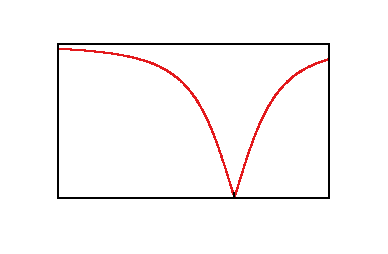
\includegraphics{./plots/resonanzkurve_ref}}%
    \gplfronttext
  \end{picture}%
\endgroup
}
			}
	\end{overpic}
\end{frame}

\begin{frame}{Messablauf}
	\addtocounter{framenumber}{-1} 
	\vspace*{2cm}
	\centering
	\begin{overpic}[width=0.95\textwidth,tics=10]{./figures/messaufbau_messpos.pdf}
		\put (45,20) {
			\fcolorbox{Black}{White}{% GNUPLOT: LaTeX picture with Postscript
\begingroup
  \makeatletter
  \providecommand\color[2][]{%
    \GenericError{(gnuplot) \space\space\space\@spaces}{%
      Package color not loaded in conjunction with
      terminal option `colourtext'%
    }{See the gnuplot documentation for explanation.%
    }{Either use 'blacktext' in gnuplot or load the package
      color.sty in LaTeX.}%
    \renewcommand\color[2][]{}%
  }%
  \providecommand\includegraphics[2][]{%
    \GenericError{(gnuplot) \space\space\space\@spaces}{%
      Package graphicx or graphics not loaded%
    }{See the gnuplot documentation for explanation.%
    }{The gnuplot epslatex terminal needs graphicx.sty or graphics.sty.}%
    \renewcommand\includegraphics[2][]{}%
  }%
  \providecommand\rotatebox[2]{#2}%
  \@ifundefined{ifGPcolor}{%
    \newif\ifGPcolor
    \GPcolortrue
  }{}%
  \@ifundefined{ifGPblacktext}{%
    \newif\ifGPblacktext
    \GPblacktexttrue
  }{}%
  % define a \g@addto@macro without @ in the name:
  \let\gplgaddtomacro\g@addto@macro
  % define empty templates for all commands taking text:
  \gdef\gplbacktext{}%
  \gdef\gplfronttext{}%
  \makeatother
  \ifGPblacktext
    % no textcolor at all
    \def\colorrgb#1{}%
    \def\colorgray#1{}%
  \else
    % gray or color?
    \ifGPcolor
      \def\colorrgb#1{\color[rgb]{#1}}%
      \def\colorgray#1{\color[gray]{#1}}%
      \expandafter\def\csname LTw\endcsname{\color{white}}%
      \expandafter\def\csname LTb\endcsname{\color{black}}%
      \expandafter\def\csname LTa\endcsname{\color{black}}%
      \expandafter\def\csname LT0\endcsname{\color[rgb]{1,0,0}}%
      \expandafter\def\csname LT1\endcsname{\color[rgb]{0,1,0}}%
      \expandafter\def\csname LT2\endcsname{\color[rgb]{0,0,1}}%
      \expandafter\def\csname LT3\endcsname{\color[rgb]{1,0,1}}%
      \expandafter\def\csname LT4\endcsname{\color[rgb]{0,1,1}}%
      \expandafter\def\csname LT5\endcsname{\color[rgb]{1,1,0}}%
      \expandafter\def\csname LT6\endcsname{\color[rgb]{0,0,0}}%
      \expandafter\def\csname LT7\endcsname{\color[rgb]{1,0.3,0}}%
      \expandafter\def\csname LT8\endcsname{\color[rgb]{0.5,0.5,0.5}}%
    \else
      % gray
      \def\colorrgb#1{\color{black}}%
      \def\colorgray#1{\color[gray]{#1}}%
      \expandafter\def\csname LTw\endcsname{\color{white}}%
      \expandafter\def\csname LTb\endcsname{\color{black}}%
      \expandafter\def\csname LTa\endcsname{\color{black}}%
      \expandafter\def\csname LT0\endcsname{\color{black}}%
      \expandafter\def\csname LT1\endcsname{\color{black}}%
      \expandafter\def\csname LT2\endcsname{\color{black}}%
      \expandafter\def\csname LT3\endcsname{\color{black}}%
      \expandafter\def\csname LT4\endcsname{\color{black}}%
      \expandafter\def\csname LT5\endcsname{\color{black}}%
      \expandafter\def\csname LT6\endcsname{\color{black}}%
      \expandafter\def\csname LT7\endcsname{\color{black}}%
      \expandafter\def\csname LT8\endcsname{\color{black}}%
    \fi
  \fi
    \setlength{\unitlength}{0.0500bp}%
    \ifx\gptboxheight\undefined%
      \newlength{\gptboxheight}%
      \newlength{\gptboxwidth}%
      \newsavebox{\gptboxtext}%
    \fi%
    \setlength{\fboxrule}{0.5pt}%
    \setlength{\fboxsep}{1pt}%
\begin{picture}(3400.00,2124.00)%
    \gplgaddtomacro\gplbacktext{%
    }%
    \gplgaddtomacro\gplfronttext{%
      \csname LTb\endcsname%
      \put(176,1116){\rotatebox{-270}{\makebox(0,0){\strut{}$|\rho|$}}}%
      \put(1699,154){\makebox(0,0){\strut{}$\omega$}}%
      \csname LTb\endcsname%
      \put(2091,285){\makebox(0,0){\strut{}\scriptsize{$\omega_0$}}}%
      \put(1700,775){\makebox(0,0){\strut{}$\Delta \omega$}}%
      \put(1308,285){\makebox(0,0){\strut{}\scriptsize{$\omega_1$}}}%
    }%
    \gplbacktext
    \put(0,0){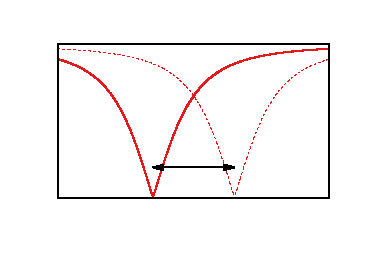
\includegraphics{./plots/resonanzkurve}}%
    \gplfronttext
  \end{picture}%
\endgroup
}
		}
	\end{overpic}
\end{frame}

\section{Ergebnisse}
\begin{frame}{Ergebnisse}
	\begin{itemize}
		\setlength\itemsep{1.25em}
		\item Vermessung verschiedener Resonatormoden	
		\begin{itemize}
			\setlength\itemsep{0.25em}
			\item $\mathrm{TM}_{010}$-Moden
			\item Moden höherer Ordnung
		\end{itemize}
		
		\item Güte $Q_0$, Koppelfaktor $\kappa$, Resonanzfrequenz $\nu_0$ aus Reflexionsspektrum
		
		\item Berechnung des el. Feldes $E_0 / \sqrt{P_\mathrm{V}}$
		\begin{itemize}
			\setlength\itemsep{0.25em}
			\item unabhängig von eingekoppelter Leistung
			\item einfache Berechnung der Shuntimpedanz:
			\begin{align*}
			R_\mathrm{S} = \frac{|U|^2}{2 P_\mathrm{V}}
			\end{align*}
			
		\end{itemize}
	\end{itemize}
\end{frame}

\begin{frame}{$\text{TM}_{010}$-$\pi$-Mode}
	\centering
	% GNUPLOT: LaTeX picture with Postscript
\begingroup
  \makeatletter
  \providecommand\color[2][]{%
    \GenericError{(gnuplot) \space\space\space\@spaces}{%
      Package color not loaded in conjunction with
      terminal option `colourtext'%
    }{See the gnuplot documentation for explanation.%
    }{Either use 'blacktext' in gnuplot or load the package
      color.sty in LaTeX.}%
    \renewcommand\color[2][]{}%
  }%
  \providecommand\includegraphics[2][]{%
    \GenericError{(gnuplot) \space\space\space\@spaces}{%
      Package graphicx or graphics not loaded%
    }{See the gnuplot documentation for explanation.%
    }{The gnuplot epslatex terminal needs graphicx.sty or graphics.sty.}%
    \renewcommand\includegraphics[2][]{}%
  }%
  \providecommand\rotatebox[2]{#2}%
  \@ifundefined{ifGPcolor}{%
    \newif\ifGPcolor
    \GPcolortrue
  }{}%
  \@ifundefined{ifGPblacktext}{%
    \newif\ifGPblacktext
    \GPblacktexttrue
  }{}%
  % define a \g@addto@macro without @ in the name:
  \let\gplgaddtomacro\g@addto@macro
  % define empty templates for all commands taking text:
  \gdef\gplbacktext{}%
  \gdef\gplfronttext{}%
  \makeatother
  \ifGPblacktext
    % no textcolor at all
    \def\colorrgb#1{}%
    \def\colorgray#1{}%
  \else
    % gray or color?
    \ifGPcolor
      \def\colorrgb#1{\color[rgb]{#1}}%
      \def\colorgray#1{\color[gray]{#1}}%
      \expandafter\def\csname LTw\endcsname{\color{white}}%
      \expandafter\def\csname LTb\endcsname{\color{black}}%
      \expandafter\def\csname LTa\endcsname{\color{black}}%
      \expandafter\def\csname LT0\endcsname{\color[rgb]{1,0,0}}%
      \expandafter\def\csname LT1\endcsname{\color[rgb]{0,1,0}}%
      \expandafter\def\csname LT2\endcsname{\color[rgb]{0,0,1}}%
      \expandafter\def\csname LT3\endcsname{\color[rgb]{1,0,1}}%
      \expandafter\def\csname LT4\endcsname{\color[rgb]{0,1,1}}%
      \expandafter\def\csname LT5\endcsname{\color[rgb]{1,1,0}}%
      \expandafter\def\csname LT6\endcsname{\color[rgb]{0,0,0}}%
      \expandafter\def\csname LT7\endcsname{\color[rgb]{1,0.3,0}}%
      \expandafter\def\csname LT8\endcsname{\color[rgb]{0.5,0.5,0.5}}%
    \else
      % gray
      \def\colorrgb#1{\color{black}}%
      \def\colorgray#1{\color[gray]{#1}}%
      \expandafter\def\csname LTw\endcsname{\color{white}}%
      \expandafter\def\csname LTb\endcsname{\color{black}}%
      \expandafter\def\csname LTa\endcsname{\color{black}}%
      \expandafter\def\csname LT0\endcsname{\color{black}}%
      \expandafter\def\csname LT1\endcsname{\color{black}}%
      \expandafter\def\csname LT2\endcsname{\color{black}}%
      \expandafter\def\csname LT3\endcsname{\color{black}}%
      \expandafter\def\csname LT4\endcsname{\color{black}}%
      \expandafter\def\csname LT5\endcsname{\color{black}}%
      \expandafter\def\csname LT6\endcsname{\color{black}}%
      \expandafter\def\csname LT7\endcsname{\color{black}}%
      \expandafter\def\csname LT8\endcsname{\color{black}}%
    \fi
  \fi
    \setlength{\unitlength}{0.0500bp}%
    \ifx\gptboxheight\undefined%
      \newlength{\gptboxheight}%
      \newlength{\gptboxwidth}%
      \newsavebox{\gptboxtext}%
    \fi%
    \setlength{\fboxrule}{0.5pt}%
    \setlength{\fboxsep}{1pt}%
\begin{picture}(6802.00,4534.00)%
    \gplgaddtomacro\gplbacktext{%
      \csname LTb\endcsname%
      \put(814,704){\makebox(0,0)[r]{\strut{}-20}}%
      \csname LTb\endcsname%
      \put(814,1383){\makebox(0,0)[r]{\strut{}-16}}%
      \csname LTb\endcsname%
      \put(814,2062){\makebox(0,0)[r]{\strut{}-12}}%
      \csname LTb\endcsname%
      \put(814,2741){\makebox(0,0)[r]{\strut{}-8}}%
      \csname LTb\endcsname%
      \put(814,3420){\makebox(0,0)[r]{\strut{}-4}}%
      \csname LTb\endcsname%
      \put(814,4099){\makebox(0,0)[r]{\strut{}0}}%
      \csname LTb\endcsname%
      \put(946,484){\makebox(0,0){\strut{}0}}%
      \csname LTb\endcsname%
      \put(2176,484){\makebox(0,0){\strut{}500}}%
      \csname LTb\endcsname%
      \put(3405,484){\makebox(0,0){\strut{}1000}}%
      \csname LTb\endcsname%
      \put(4635,484){\makebox(0,0){\strut{}1500}}%
      \csname LTb\endcsname%
      \put(5864,484){\makebox(0,0){\strut{}2000}}%
    }%
    \gplgaddtomacro\gplfronttext{%
      \csname LTb\endcsname%
      \put(176,2486){\rotatebox{-270}{\makebox(0,0){\strut{}$\Delta \nu$ / \si{\kilo\hertz}}}}%
      \put(3675,154){\makebox(0,0){\strut{}$z$ / \si{mm}}}%
    }%
    \gplbacktext
    \put(0,0){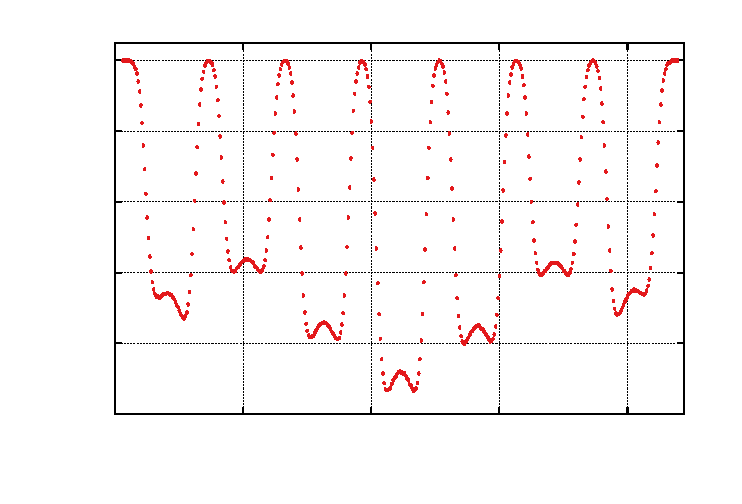
\includegraphics{./plots/frequenzverschiebung}}%
    \gplfronttext
  \end{picture}%
\endgroup

\end{frame}
\begin{frame}{$\text{TM}_{010}$-$\pi$-Mode}
	\centering
	% GNUPLOT: LaTeX picture with Postscript
\begingroup
  \makeatletter
  \providecommand\color[2][]{%
    \GenericError{(gnuplot) \space\space\space\@spaces}{%
      Package color not loaded in conjunction with
      terminal option `colourtext'%
    }{See the gnuplot documentation for explanation.%
    }{Either use 'blacktext' in gnuplot or load the package
      color.sty in LaTeX.}%
    \renewcommand\color[2][]{}%
  }%
  \providecommand\includegraphics[2][]{%
    \GenericError{(gnuplot) \space\space\space\@spaces}{%
      Package graphicx or graphics not loaded%
    }{See the gnuplot documentation for explanation.%
    }{The gnuplot epslatex terminal needs graphicx.sty or graphics.sty.}%
    \renewcommand\includegraphics[2][]{}%
  }%
  \providecommand\rotatebox[2]{#2}%
  \@ifundefined{ifGPcolor}{%
    \newif\ifGPcolor
    \GPcolortrue
  }{}%
  \@ifundefined{ifGPblacktext}{%
    \newif\ifGPblacktext
    \GPblacktexttrue
  }{}%
  % define a \g@addto@macro without @ in the name:
  \let\gplgaddtomacro\g@addto@macro
  % define empty templates for all commands taking text:
  \gdef\gplbacktext{}%
  \gdef\gplfronttext{}%
  \makeatother
  \ifGPblacktext
    % no textcolor at all
    \def\colorrgb#1{}%
    \def\colorgray#1{}%
  \else
    % gray or color?
    \ifGPcolor
      \def\colorrgb#1{\color[rgb]{#1}}%
      \def\colorgray#1{\color[gray]{#1}}%
      \expandafter\def\csname LTw\endcsname{\color{white}}%
      \expandafter\def\csname LTb\endcsname{\color{black}}%
      \expandafter\def\csname LTa\endcsname{\color{black}}%
      \expandafter\def\csname LT0\endcsname{\color[rgb]{1,0,0}}%
      \expandafter\def\csname LT1\endcsname{\color[rgb]{0,1,0}}%
      \expandafter\def\csname LT2\endcsname{\color[rgb]{0,0,1}}%
      \expandafter\def\csname LT3\endcsname{\color[rgb]{1,0,1}}%
      \expandafter\def\csname LT4\endcsname{\color[rgb]{0,1,1}}%
      \expandafter\def\csname LT5\endcsname{\color[rgb]{1,1,0}}%
      \expandafter\def\csname LT6\endcsname{\color[rgb]{0,0,0}}%
      \expandafter\def\csname LT7\endcsname{\color[rgb]{1,0.3,0}}%
      \expandafter\def\csname LT8\endcsname{\color[rgb]{0.5,0.5,0.5}}%
    \else
      % gray
      \def\colorrgb#1{\color{black}}%
      \def\colorgray#1{\color[gray]{#1}}%
      \expandafter\def\csname LTw\endcsname{\color{white}}%
      \expandafter\def\csname LTb\endcsname{\color{black}}%
      \expandafter\def\csname LTa\endcsname{\color{black}}%
      \expandafter\def\csname LT0\endcsname{\color{black}}%
      \expandafter\def\csname LT1\endcsname{\color{black}}%
      \expandafter\def\csname LT2\endcsname{\color{black}}%
      \expandafter\def\csname LT3\endcsname{\color{black}}%
      \expandafter\def\csname LT4\endcsname{\color{black}}%
      \expandafter\def\csname LT5\endcsname{\color{black}}%
      \expandafter\def\csname LT6\endcsname{\color{black}}%
      \expandafter\def\csname LT7\endcsname{\color{black}}%
      \expandafter\def\csname LT8\endcsname{\color{black}}%
    \fi
  \fi
    \setlength{\unitlength}{0.0500bp}%
    \ifx\gptboxheight\undefined%
      \newlength{\gptboxheight}%
      \newlength{\gptboxwidth}%
      \newsavebox{\gptboxtext}%
    \fi%
    \setlength{\fboxrule}{0.5pt}%
    \setlength{\fboxsep}{1pt}%
\begin{picture}(6802.00,4534.00)%
    \gplgaddtomacro\gplbacktext{%
      \csname LTb\endcsname%
      \put(946,914){\makebox(0,0)[r]{\strut{}0}}%
      \csname LTb\endcsname%
      \put(946,1333){\makebox(0,0)[r]{\strut{}1000}}%
      \csname LTb\endcsname%
      \put(946,1753){\makebox(0,0)[r]{\strut{}2000}}%
      \csname LTb\endcsname%
      \put(946,2172){\makebox(0,0)[r]{\strut{}3000}}%
      \csname LTb\endcsname%
      \put(946,2591){\makebox(0,0)[r]{\strut{}4000}}%
      \csname LTb\endcsname%
      \put(946,3011){\makebox(0,0)[r]{\strut{}5000}}%
      \csname LTb\endcsname%
      \put(946,3430){\makebox(0,0)[r]{\strut{}6000}}%
      \csname LTb\endcsname%
      \put(946,3850){\makebox(0,0)[r]{\strut{}7000}}%
      \csname LTb\endcsname%
      \put(946,4269){\makebox(0,0)[r]{\strut{}8000}}%
      \csname LTb\endcsname%
      \put(1078,484){\makebox(0,0){\strut{}0}}%
      \csname LTb\endcsname%
      \put(2278,484){\makebox(0,0){\strut{}500}}%
      \csname LTb\endcsname%
      \put(3478,484){\makebox(0,0){\strut{}1000}}%
      \csname LTb\endcsname%
      \put(4677,484){\makebox(0,0){\strut{}1500}}%
      \csname LTb\endcsname%
      \put(5877,484){\makebox(0,0){\strut{}2000}}%
    }%
    \gplgaddtomacro\gplfronttext{%
      \csname LTb\endcsname%
      \put(176,2486){\rotatebox{-270}{\makebox(0,0){\strut{}$\frac{E_0(z)}{\sqrt{P_\mathrm{V}}}$ / \si{\volt\per\metre\per\watt\tothe{0{,}5}}}}}%
      \put(3741,154){\makebox(0,0){\strut{}$z$ / \si{mm}}}%
      \csname LTb\endcsname%
      \put(5682,4096){\makebox(0,0)[r]{\strut{}Amplitude}}%
      \csname LTb\endcsname%
      \put(5682,3876){\makebox(0,0)[r]{\strut{}effektives Feld}}%
    }%
    \gplbacktext
    \put(0,0){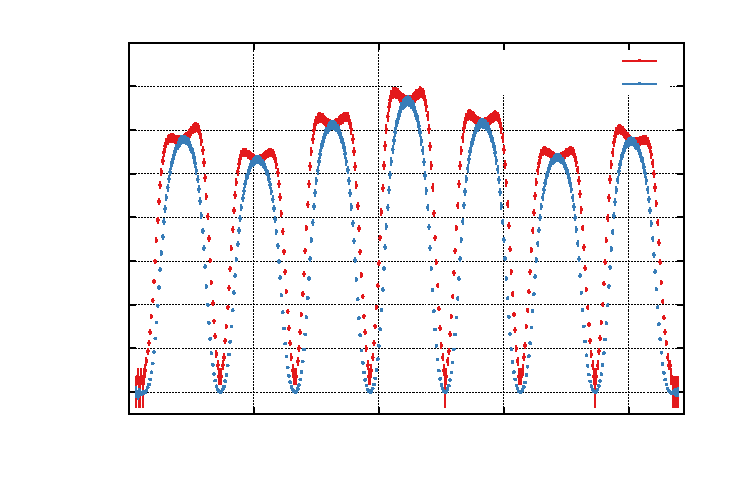
\includegraphics{./plots/messung_pi_1}}%
    \gplfronttext
  \end{picture}%
\endgroup

\end{frame}
\begin{frame}{$\text{TM}_{010}$-$\pi$-Mode}
	\addtocounter{framenumber}{-1}
	\centering
	% GNUPLOT: LaTeX picture with Postscript
\begingroup
  \makeatletter
  \providecommand\color[2][]{%
    \GenericError{(gnuplot) \space\space\space\@spaces}{%
      Package color not loaded in conjunction with
      terminal option `colourtext'%
    }{See the gnuplot documentation for explanation.%
    }{Either use 'blacktext' in gnuplot or load the package
      color.sty in LaTeX.}%
    \renewcommand\color[2][]{}%
  }%
  \providecommand\includegraphics[2][]{%
    \GenericError{(gnuplot) \space\space\space\@spaces}{%
      Package graphicx or graphics not loaded%
    }{See the gnuplot documentation for explanation.%
    }{The gnuplot epslatex terminal needs graphicx.sty or graphics.sty.}%
    \renewcommand\includegraphics[2][]{}%
  }%
  \providecommand\rotatebox[2]{#2}%
  \@ifundefined{ifGPcolor}{%
    \newif\ifGPcolor
    \GPcolortrue
  }{}%
  \@ifundefined{ifGPblacktext}{%
    \newif\ifGPblacktext
    \GPblacktexttrue
  }{}%
  % define a \g@addto@macro without @ in the name:
  \let\gplgaddtomacro\g@addto@macro
  % define empty templates for all commands taking text:
  \gdef\gplbacktext{}%
  \gdef\gplfronttext{}%
  \makeatother
  \ifGPblacktext
    % no textcolor at all
    \def\colorrgb#1{}%
    \def\colorgray#1{}%
  \else
    % gray or color?
    \ifGPcolor
      \def\colorrgb#1{\color[rgb]{#1}}%
      \def\colorgray#1{\color[gray]{#1}}%
      \expandafter\def\csname LTw\endcsname{\color{white}}%
      \expandafter\def\csname LTb\endcsname{\color{black}}%
      \expandafter\def\csname LTa\endcsname{\color{black}}%
      \expandafter\def\csname LT0\endcsname{\color[rgb]{1,0,0}}%
      \expandafter\def\csname LT1\endcsname{\color[rgb]{0,1,0}}%
      \expandafter\def\csname LT2\endcsname{\color[rgb]{0,0,1}}%
      \expandafter\def\csname LT3\endcsname{\color[rgb]{1,0,1}}%
      \expandafter\def\csname LT4\endcsname{\color[rgb]{0,1,1}}%
      \expandafter\def\csname LT5\endcsname{\color[rgb]{1,1,0}}%
      \expandafter\def\csname LT6\endcsname{\color[rgb]{0,0,0}}%
      \expandafter\def\csname LT7\endcsname{\color[rgb]{1,0.3,0}}%
      \expandafter\def\csname LT8\endcsname{\color[rgb]{0.5,0.5,0.5}}%
    \else
      % gray
      \def\colorrgb#1{\color{black}}%
      \def\colorgray#1{\color[gray]{#1}}%
      \expandafter\def\csname LTw\endcsname{\color{white}}%
      \expandafter\def\csname LTb\endcsname{\color{black}}%
      \expandafter\def\csname LTa\endcsname{\color{black}}%
      \expandafter\def\csname LT0\endcsname{\color{black}}%
      \expandafter\def\csname LT1\endcsname{\color{black}}%
      \expandafter\def\csname LT2\endcsname{\color{black}}%
      \expandafter\def\csname LT3\endcsname{\color{black}}%
      \expandafter\def\csname LT4\endcsname{\color{black}}%
      \expandafter\def\csname LT5\endcsname{\color{black}}%
      \expandafter\def\csname LT6\endcsname{\color{black}}%
      \expandafter\def\csname LT7\endcsname{\color{black}}%
      \expandafter\def\csname LT8\endcsname{\color{black}}%
    \fi
  \fi
    \setlength{\unitlength}{0.0500bp}%
    \ifx\gptboxheight\undefined%
      \newlength{\gptboxheight}%
      \newlength{\gptboxwidth}%
      \newsavebox{\gptboxtext}%
    \fi%
    \setlength{\fboxrule}{0.5pt}%
    \setlength{\fboxsep}{1pt}%
\begin{picture}(6802.00,4534.00)%
    \gplgaddtomacro\gplbacktext{%
      \csname LTb\endcsname%
      \put(946,914){\makebox(0,0)[r]{\strut{}0}}%
      \csname LTb\endcsname%
      \put(946,1753){\makebox(0,0)[r]{\strut{}2000}}%
      \csname LTb\endcsname%
      \put(946,2591){\makebox(0,0)[r]{\strut{}4000}}%
      \csname LTb\endcsname%
      \put(946,3430){\makebox(0,0)[r]{\strut{}6000}}%
      \csname LTb\endcsname%
      \put(946,4269){\makebox(0,0)[r]{\strut{}8000}}%
      \csname LTb\endcsname%
      \put(1078,484){\makebox(0,0){\strut{}0}}%
      \csname LTb\endcsname%
      \put(2278,484){\makebox(0,0){\strut{}500}}%
      \csname LTb\endcsname%
      \put(3478,484){\makebox(0,0){\strut{}1000}}%
      \csname LTb\endcsname%
      \put(4677,484){\makebox(0,0){\strut{}1500}}%
      \csname LTb\endcsname%
      \put(5877,484){\makebox(0,0){\strut{}2000}}%
    }%
    \gplgaddtomacro\gplfronttext{%
      \csname LTb\endcsname%
      \put(176,2486){\rotatebox{-270}{\makebox(0,0){\strut{}$\frac{E_0(z)}{\sqrt{P_\mathrm{V}}}$ / \si{\volt\per\metre\per\watt\tothe{0{,}5}}}}}%
      \put(3741,154){\makebox(0,0){\strut{}$z$ / \si{mm}}}%
      \csname LTb\endcsname%
      \put(5682,4096){\makebox(0,0)[r]{\strut{}Amplitude}}%
      \csname LTb\endcsname%
      \put(5682,3876){\makebox(0,0)[r]{\strut{}effektives Feld}}%
    }%
    \gplbacktext
    \put(0,0){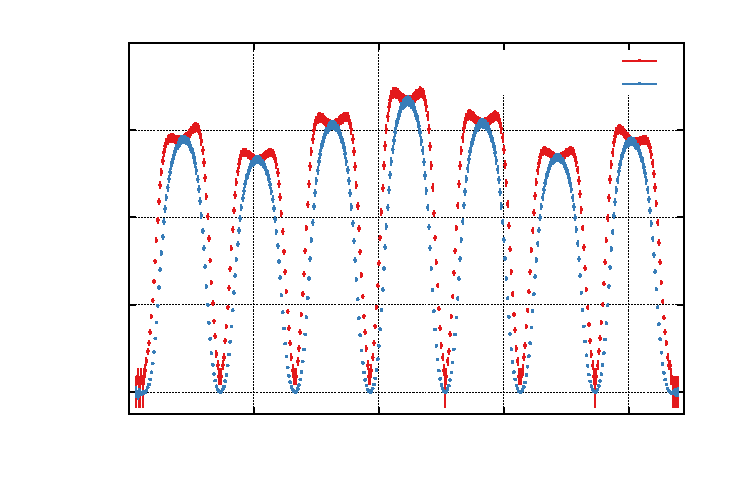
\includegraphics{./plots/messung_pi_2}}%
    \gplfronttext
  \end{picture}%
\endgroup

\end{frame}

\begin{frame}
	\centering
	{\def\arraystretch{2}\tabcolsep=10pt
	\begin{tabular}{p{3.5cm}|cc} \toprule
		$\mathrm{TM}_{010}$-$\pi$-Mode & \textbf{PETRA-III} & \textbf{PETRA-IV} \\ \midrule
		Kreisgüte $Q_0$ & \num{29560 +- 110} & \num{28200 +- 180} \\
		Shuntimpedanz $R_\mathrm{S}$ & \SI{25.7 +- 1.0}{\mega\ohm} & \SI{24.5 +- 0.9}{\mega\ohm} \\
		Beschleunigungs\-spannung~$U$\newline($P_\mathrm{V} = \SI{100}{\kilo\watt}$)& \SI{2.27 +- 0.05}{\mega\volt} & \SI{2.21 +- 0.04}{\mega\volt} \\
	\end{tabular}
	}
	\vspace*{0.5cm}
	\begin{itemize}
		\item \textbf{Vergleich:} fünfzellige PETRA-Resonatoren (\SI{100}{kW}) \cite{desy_petra5}
		\begin{align*}
			R_\mathrm{S} \approx \SI{15}{\mega\ohm} \qquad U \approx \SI{1.7}{\mega\volt}
		\end{align*}
	\end{itemize}
\end{frame}

\begin{frame}{Moden höherer Ordnung}
	\begin{itemize}
		\setlength\itemsep{1.25em}
		\item unbegrenzte Anzahl von Moden höherer Ordnung
		\begin{itemize}
			\item Vorauswahl durch Simulationen \cite{schedler} und Güte
		\end{itemize}
		
		\item \textbf{Erwartung:} hohe Shuntimpedanz einer $\mathrm{TM}_{021}$-Mode
		\begin{itemize}
			\item größte Shuntimpedanz dieser Moden:
			\begin{align*}
			\nu_0 = \SI{1465.8}{\mega\hertz}\qquad R_\mathrm{S} = \SI{183.0 +- 6.4}{\kilo\ohm}
			\end{align*}
			\item zwei Größenordnungen unter der Beschleunigermode
		\end{itemize}
		
		\item höchste gemessene Shuntimpedanz:
		\begin{align*}
			\mathrm{TE}_{111}: \quad \nu_0 = \SI{702.7}{\mega\hertz} \qquad R_\mathrm{S} = \SI{326 +- 11}{\kilo\ohm}
		\end{align*}
	\end{itemize}
\end{frame}


\begin{frame}{Zusammenfassung}
	\begin{itemize}
		\setlength\itemsep{1.25em}
		\item zuverlässige Methode zur Feldvermessung
		
		\item $\mathrm{TM}_{010}$-Mode beider Resonatoren erfüllt die Erwartungen
		
		\item keine Moden höherer Ordnung mit hoher Shuntimpedanz identifiziert
		\begin{itemize}
			\item Einfluss auf Instabilitäten
		\end{itemize}
	\end{itemize}
\end{frame}

\begin{frame}{Quellen}
	\begin{thebibliography}{9}
		\bibitem{desy_petra7}
		DESY-MHFe,
		\emph{Data Sheet: 500 MHz, 7-Cell Cavity}
		
		\bibitem{desy_petra5}
		DESY-MHFe,
		\emph{Data Sheet: 500 MHz, 5-Cell Cavity}
		
		\bibitem{schedler}
		M.\ Schedler et al.,
		\emph{A New RF station for the ELSA Stretcher Ring},
		IPAC'15 Conf.\ Proc.\ (2015)
		
			
	\end{thebibliography}
	
\end{frame}

\beginbackup
% Hier die Backupfolien

\begin{frame}
	\centering
	\textbf{Zusätzliche Folien:}
\end{frame}

\begin{frame}{Resonatormoden $\mathrm{TM}_{m10}$}
	\begin{columns}[T]
		\column{0.5\textwidth}
		\begin{figure}[h]
			\centering
			\hspace*{0.70cm}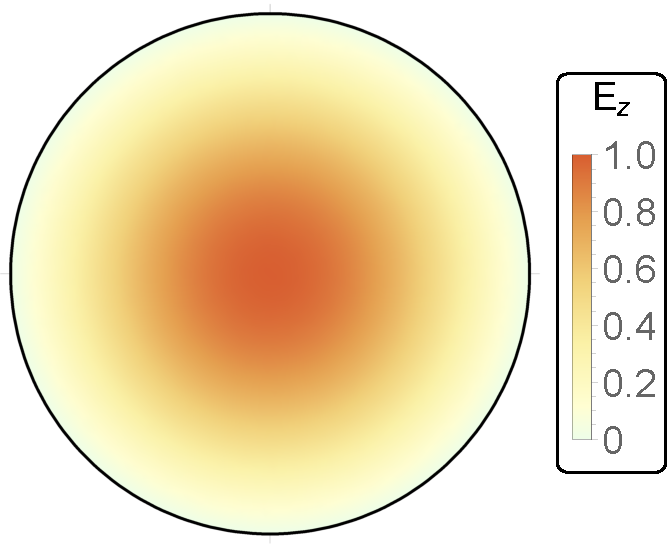
\includegraphics[scale=0.4]{./figures/tm010.pdf}
			\vspace*{-0.2cm}
			\caption{$\mathrm{TM}_{010}$}
		\end{figure}
		
		\column{0.5\textwidth}
		\begin{figure}[h]
			\centering
			\hspace*{0.70cm}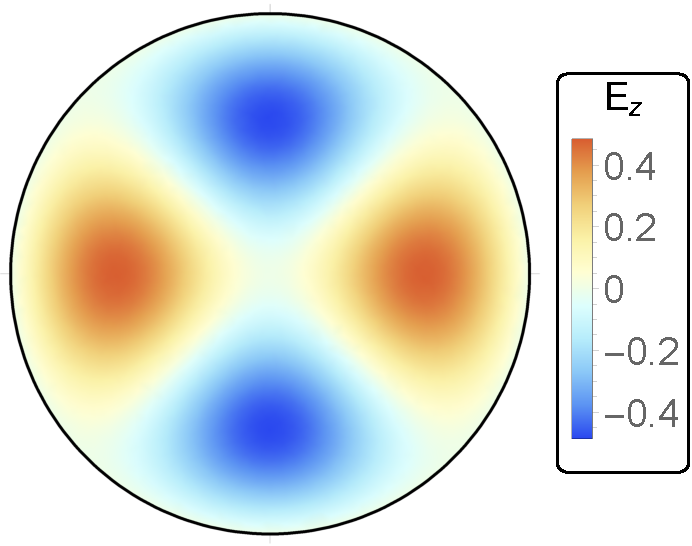
\includegraphics[scale=0.4]{./figures/tm210.pdf}
			\vspace*{-0.2cm}
			\caption{$\mathrm{TM}_{210}$}
		\end{figure}
	\end{columns}
	\vfill
	\begin{itemize}
		\item $\mathrm{TM}_{mnp}$ / $\mathrm{TE}_{mnp}$:
		\begin{itemize}
			\setlength\itemsep{0.25em}
			\item $m$: azimuthale Perioden
			\item $n$: radiale Knoten
			\item $p$: halbe longitudinale Perioden
		\end{itemize}
	\end{itemize}
\end{frame}

\begin{frame}{Resonatormoden $\mathrm{TM}_{01p}$}
	\centering
	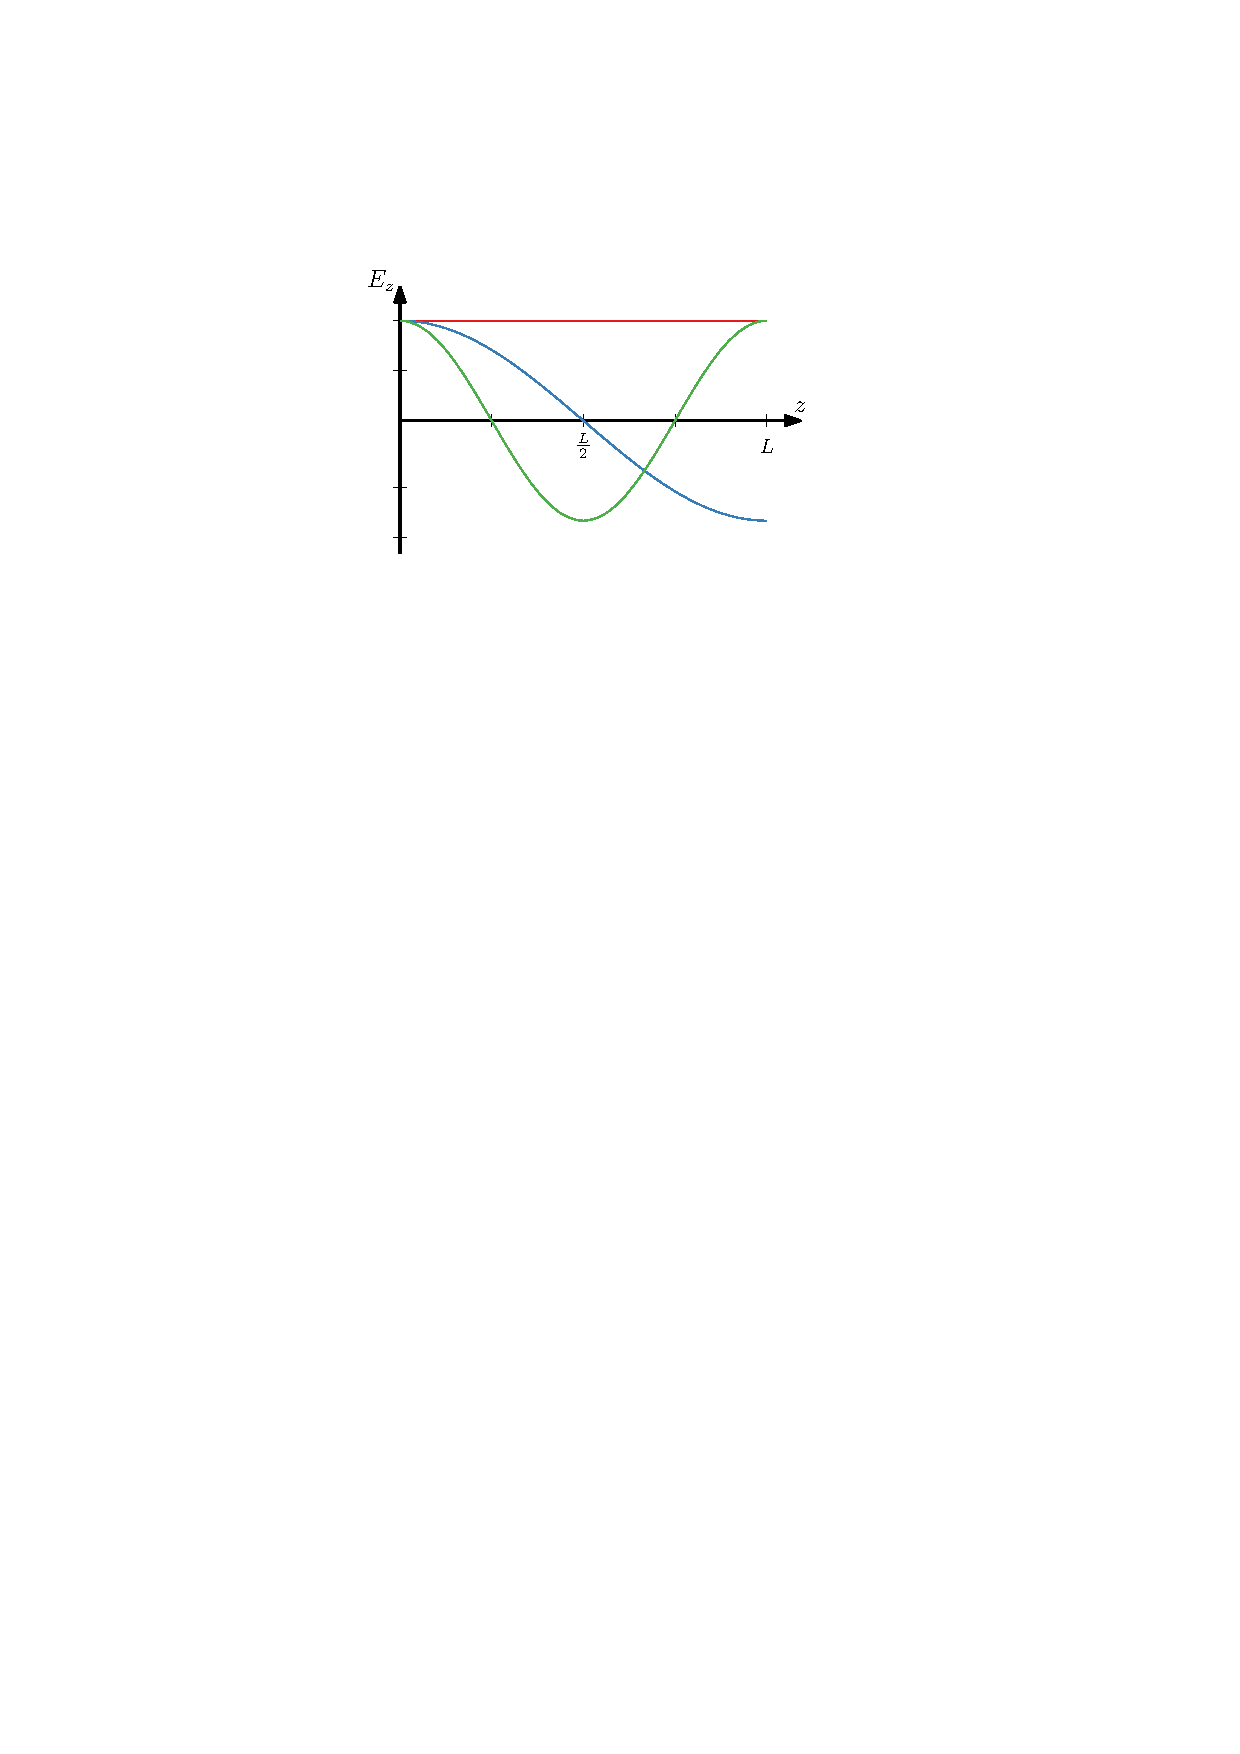
\includegraphics[scale=1.0]{./figures/longitudinale_periode.pdf}
\end{frame}

\begin{frame}{Resonanzkurven}
	\begin{small}
		\centering
		% GNUPLOT: LaTeX picture with Postscript
\begingroup
  \makeatletter
  \providecommand\color[2][]{%
    \GenericError{(gnuplot) \space\space\space\@spaces}{%
      Package color not loaded in conjunction with
      terminal option `colourtext'%
    }{See the gnuplot documentation for explanation.%
    }{Either use 'blacktext' in gnuplot or load the package
      color.sty in LaTeX.}%
    \renewcommand\color[2][]{}%
  }%
  \providecommand\includegraphics[2][]{%
    \GenericError{(gnuplot) \space\space\space\@spaces}{%
      Package graphicx or graphics not loaded%
    }{See the gnuplot documentation for explanation.%
    }{The gnuplot epslatex terminal needs graphicx.sty or graphics.sty.}%
    \renewcommand\includegraphics[2][]{}%
  }%
  \providecommand\rotatebox[2]{#2}%
  \@ifundefined{ifGPcolor}{%
    \newif\ifGPcolor
    \GPcolortrue
  }{}%
  \@ifundefined{ifGPblacktext}{%
    \newif\ifGPblacktext
    \GPblacktexttrue
  }{}%
  % define a \g@addto@macro without @ in the name:
  \let\gplgaddtomacro\g@addto@macro
  % define empty templates for all commands taking text:
  \gdef\gplbacktext{}%
  \gdef\gplfronttext{}%
  \makeatother
  \ifGPblacktext
    % no textcolor at all
    \def\colorrgb#1{}%
    \def\colorgray#1{}%
  \else
    % gray or color?
    \ifGPcolor
      \def\colorrgb#1{\color[rgb]{#1}}%
      \def\colorgray#1{\color[gray]{#1}}%
      \expandafter\def\csname LTw\endcsname{\color{white}}%
      \expandafter\def\csname LTb\endcsname{\color{black}}%
      \expandafter\def\csname LTa\endcsname{\color{black}}%
      \expandafter\def\csname LT0\endcsname{\color[rgb]{1,0,0}}%
      \expandafter\def\csname LT1\endcsname{\color[rgb]{0,1,0}}%
      \expandafter\def\csname LT2\endcsname{\color[rgb]{0,0,1}}%
      \expandafter\def\csname LT3\endcsname{\color[rgb]{1,0,1}}%
      \expandafter\def\csname LT4\endcsname{\color[rgb]{0,1,1}}%
      \expandafter\def\csname LT5\endcsname{\color[rgb]{1,1,0}}%
      \expandafter\def\csname LT6\endcsname{\color[rgb]{0,0,0}}%
      \expandafter\def\csname LT7\endcsname{\color[rgb]{1,0.3,0}}%
      \expandafter\def\csname LT8\endcsname{\color[rgb]{0.5,0.5,0.5}}%
    \else
      % gray
      \def\colorrgb#1{\color{black}}%
      \def\colorgray#1{\color[gray]{#1}}%
      \expandafter\def\csname LTw\endcsname{\color{white}}%
      \expandafter\def\csname LTb\endcsname{\color{black}}%
      \expandafter\def\csname LTa\endcsname{\color{black}}%
      \expandafter\def\csname LT0\endcsname{\color{black}}%
      \expandafter\def\csname LT1\endcsname{\color{black}}%
      \expandafter\def\csname LT2\endcsname{\color{black}}%
      \expandafter\def\csname LT3\endcsname{\color{black}}%
      \expandafter\def\csname LT4\endcsname{\color{black}}%
      \expandafter\def\csname LT5\endcsname{\color{black}}%
      \expandafter\def\csname LT6\endcsname{\color{black}}%
      \expandafter\def\csname LT7\endcsname{\color{black}}%
      \expandafter\def\csname LT8\endcsname{\color{black}}%
    \fi
  \fi
    \setlength{\unitlength}{0.0500bp}%
    \ifx\gptboxheight\undefined%
      \newlength{\gptboxheight}%
      \newlength{\gptboxwidth}%
      \newsavebox{\gptboxtext}%
    \fi%
    \setlength{\fboxrule}{0.5pt}%
    \setlength{\fboxsep}{1pt}%
\begin{picture}(6802.00,4534.00)%
    \gplgaddtomacro\gplbacktext{%
      \csname LTb\endcsname%
      \put(814,704){\makebox(0,0)[r]{\strut{}0{,}0}}%
      \put(814,1417){\makebox(0,0)[r]{\strut{}0{,}2}}%
      \put(814,2130){\makebox(0,0)[r]{\strut{}0{,}4}}%
      \put(814,2843){\makebox(0,0)[r]{\strut{}0{,}6}}%
      \put(814,3556){\makebox(0,0)[r]{\strut{}0{,}8}}%
      \put(814,4269){\makebox(0,0)[r]{\strut{}1{,}0}}%
      \put(946,484){\makebox(0,0){\strut{}0{,}99}}%
      \put(3676,484){\makebox(0,0){\strut{}1{,}00}}%
      \put(6405,484){\makebox(0,0){\strut{}1{,}01}}%
    }%
    \gplgaddtomacro\gplfronttext{%
      \csname LTb\endcsname%
      \put(176,2486){\rotatebox{-270}{\makebox(0,0){\strut{}$|\rho|$}}}%
      \put(3675,154){\makebox(0,0){\strut{}$\frac{\omega}{\omega_0}$}}%
      \csname LTb\endcsname%
      \put(5682,1537){\makebox(0,0)[r]{\strut{}$Q_0 = 500, \kappa = 1{,}0$}}%
      \csname LTb\endcsname%
      \put(5682,1317){\makebox(0,0)[r]{\strut{}$Q_0 = 250, \kappa = 1{,}0$}}%
      \csname LTb\endcsname%
      \put(5682,1097){\makebox(0,0)[r]{\strut{}$Q_0 = 500, \kappa = 0{,}5$}}%
      \csname LTb\endcsname%
      \put(5682,877){\makebox(0,0)[r]{\strut{}$Q_0 = 500, \kappa = 2{,}0$}}%
    }%
    \gplbacktext
    \put(0,0){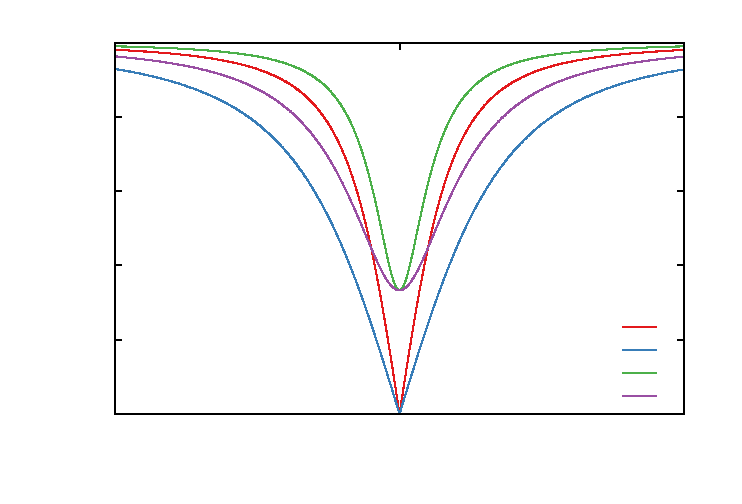
\includegraphics{./plots/resonanzkurve_full}}%
    \gplfronttext
  \end{picture}%
\endgroup

	\end{small}
\end{frame}

\begin{frame}{Störkörperkonstante $\alpha_\mathrm{s}$}
	\begin{itemize}
		\item Polarisation einer dielektrischen Kugel im homogenen el.\ Feld:
		\begin{align*}
			  \vec{P} = 3 \, \frac{\varepsilon_\mathrm{r} - 1}{\varepsilon_\mathrm{r} + 2} \, \varepsilon_0 \vec{E}_0
		\end{align*}
		
		\item resultierende Störkörperkonstante:
		\begin{align*}
			\alpha_\mathrm{s} = 3 \, \frac{\varepsilon_\mathrm{r} - 1}{\varepsilon_\mathrm{r} + 2} \, \varepsilon_0 V_\mathrm{s}
		\end{align*}
	\end{itemize}
\end{frame}

\begin{frame}{Moden einer Resonatorkette}
	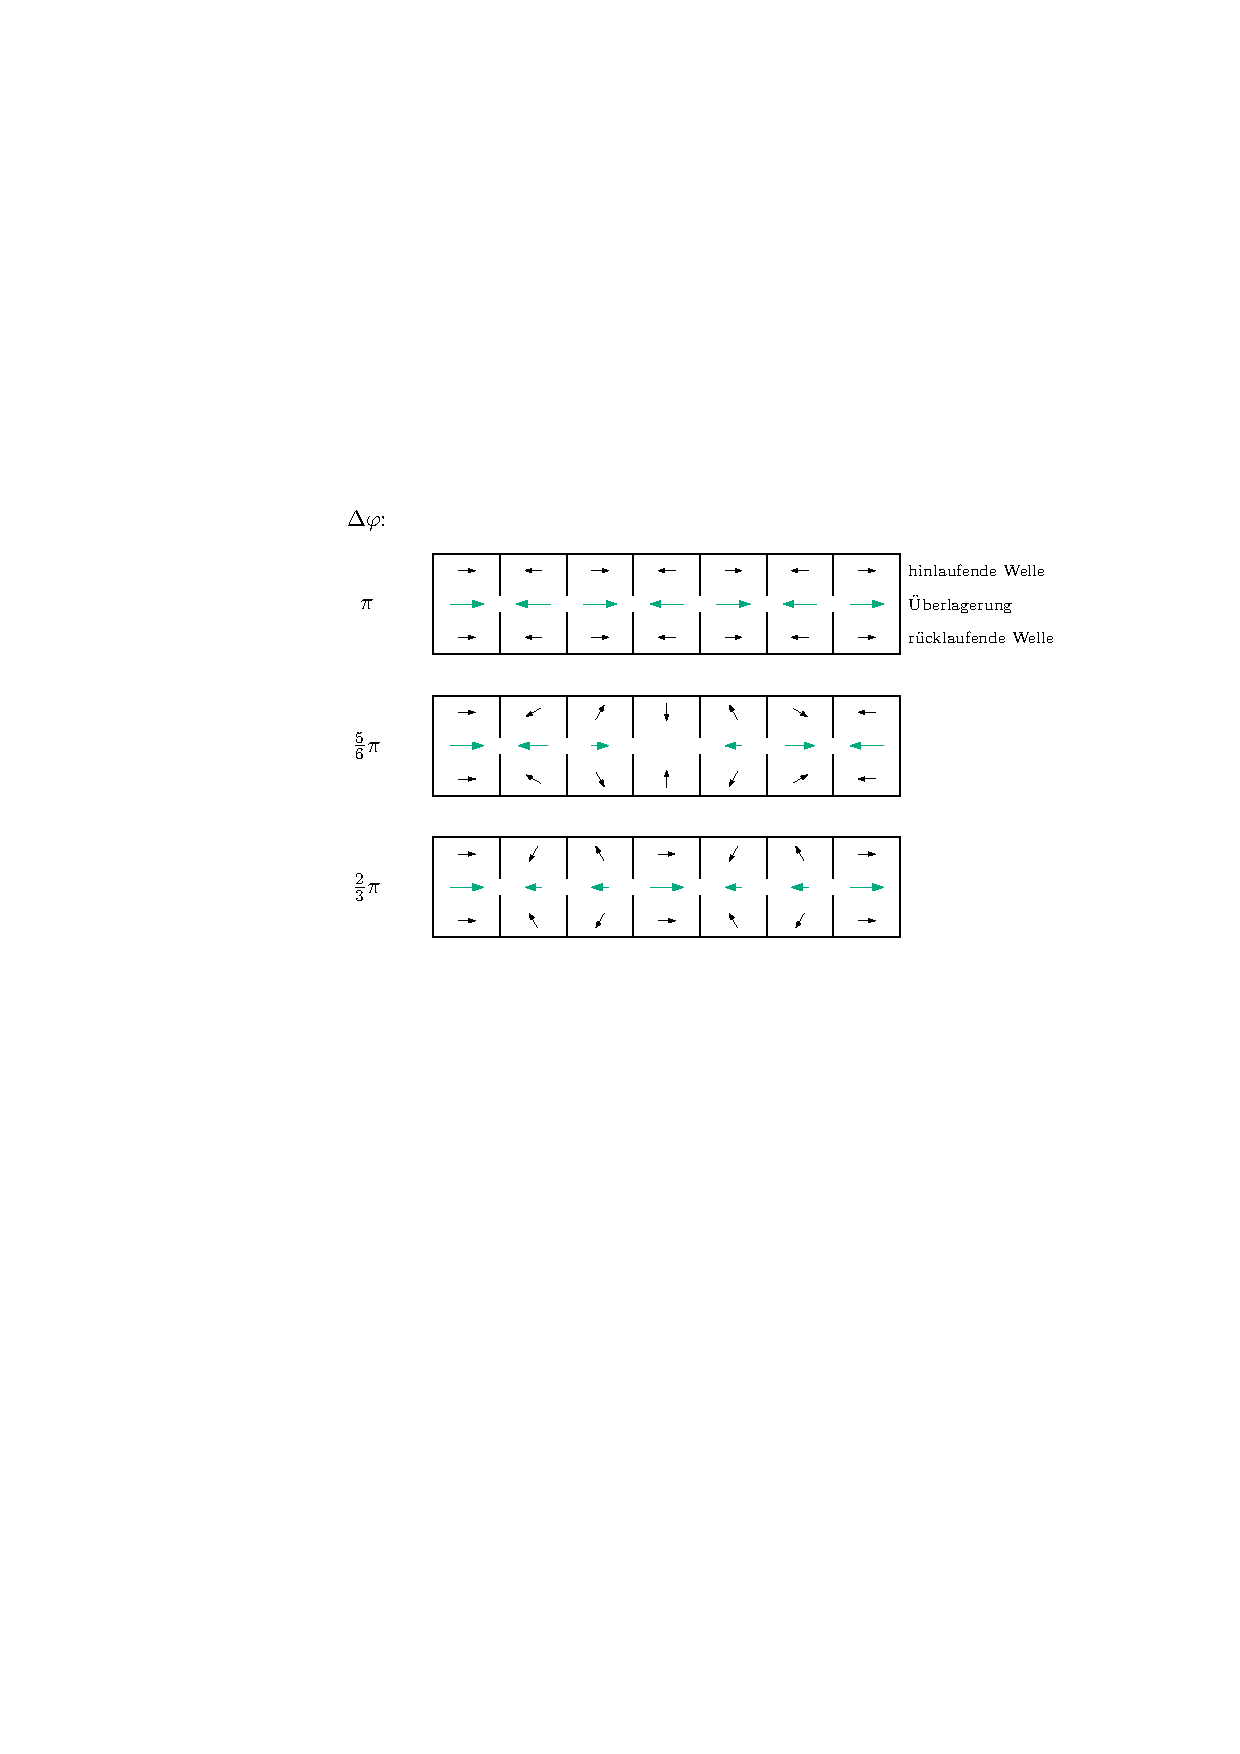
\includegraphics[scale=0.9]{./figures/phasoren_top.pdf}
\end{frame}

\begin{frame}
	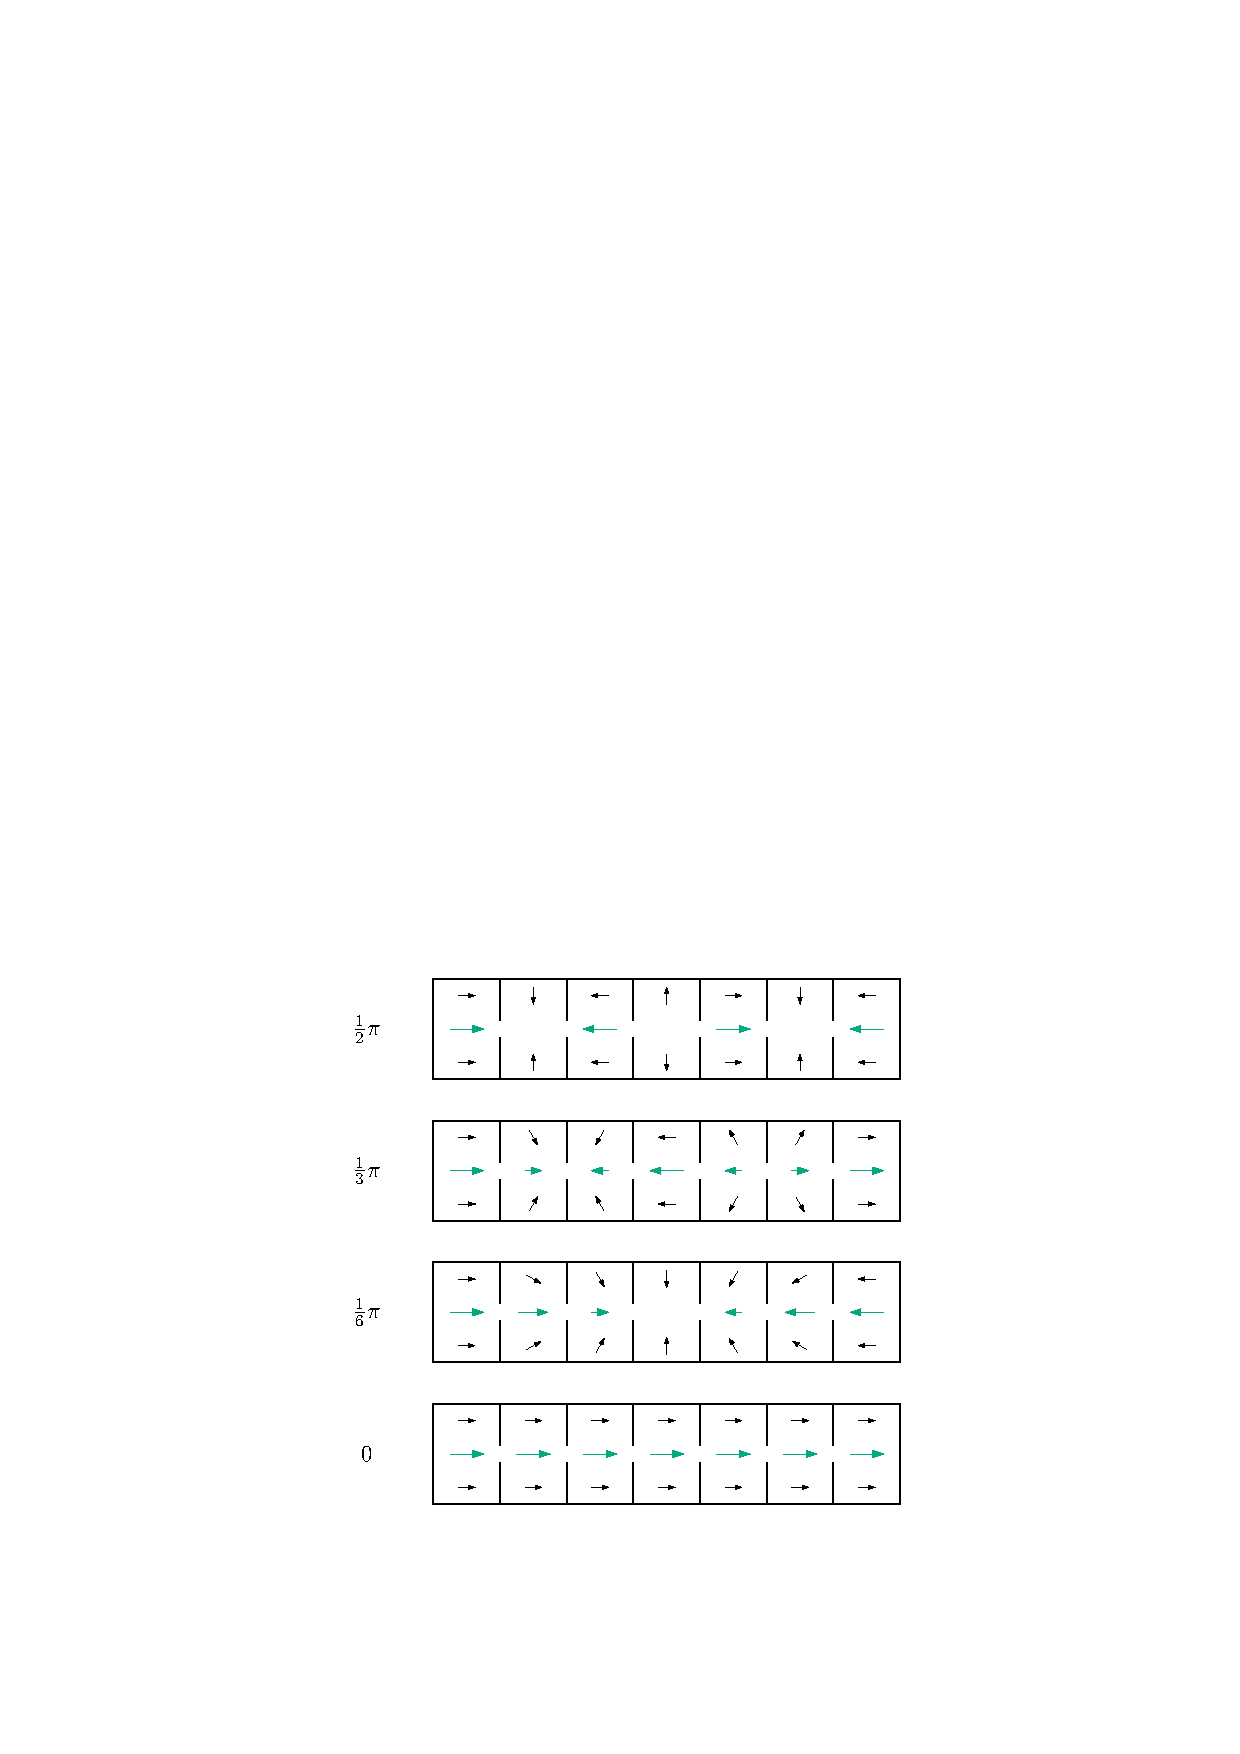
\includegraphics[scale=0.9]{./figures/phasoren_bottom.pdf}
\end{frame}
\backupend

\end{document}